\documentclass{report}

\usepackage[utf8]{inputenc} % Charakter-Kodierung
\usepackage[german]{babel} % Sprache

\usepackage[table,xcdraw]{xcolor} % Tabellen Farben
\usepackage{tabularx} % Dynamische Tabellenbreite
\usepackage{tcolorbox} % Graue Boxen
\usepackage{hyperref} % url Umgebung
\usepackage{todonotes} % Notizen
\usepackage{natbib} % Bibliographie
\usepackage{fancyhdr} % Header und Footer
\usepackage{multirow} % Multizeile
\usepackage{geometry} % Page layout
\usepackage{color} % Text Farben
\usepackage{svg} % SVG Grafiken

% Page layout
\geometry{
	bottom=3.5cm,
	headheight=180pt
}

% Nummerierung der ersten Seiten verhindern
\pagenumbering{gobble}

% Bibstyle
\bibliographystyle{plain}

% Header / Footer
\fancypagestyle{plain}{
	\fancyhf{}% Clear header/footer
	\fancyhead[R]{
\includegraphics[width=4cm]{img/cau-logo-2017}} % Rechter header
	\fancyhead[L]{\leftmark} % Linker header
	\fancyfoot[R]{\thepage} % Rechter footer
	\fancyfoot[L]{
\includegraphics[width=1cm]{img/se-logo}} % Linker footer	
}
\pagestyle{plain}

\renewcommand{\headrulewidth}{0.5pt} % Unnötige Informationen der Kapitelangabe
\renewcommand{\footrulewidth}{0.2pt} % entfernen
\renewcommand{\chaptermark}[1]{\markboth{{#1}}{}}




% Zahlen für Fußnoten
\renewcommand{\thefootnote}{\arabic{footnote}}
\renewcommand{\thempfootnote}{\arabic{mpfootnote}}

%%%%% Ausfüllen %%%%%

% Gruppenname
\newcommand{\gruppenname}{Gruppe LMS2 UE1}

% Projektname
\newcommand{\projektname}{Smart Building Solutions}

% Semester
\newcommand{\semester}{Sommer 2021}



% Titelseite

\title{
	\vspace*{-3cm}
	Pflichtenheft\\
	\projektname\\
	-\\
	\color{gray}
	Softwareprojekt \semester\\
	\gruppenname\\
	\vspace*{5mm}
	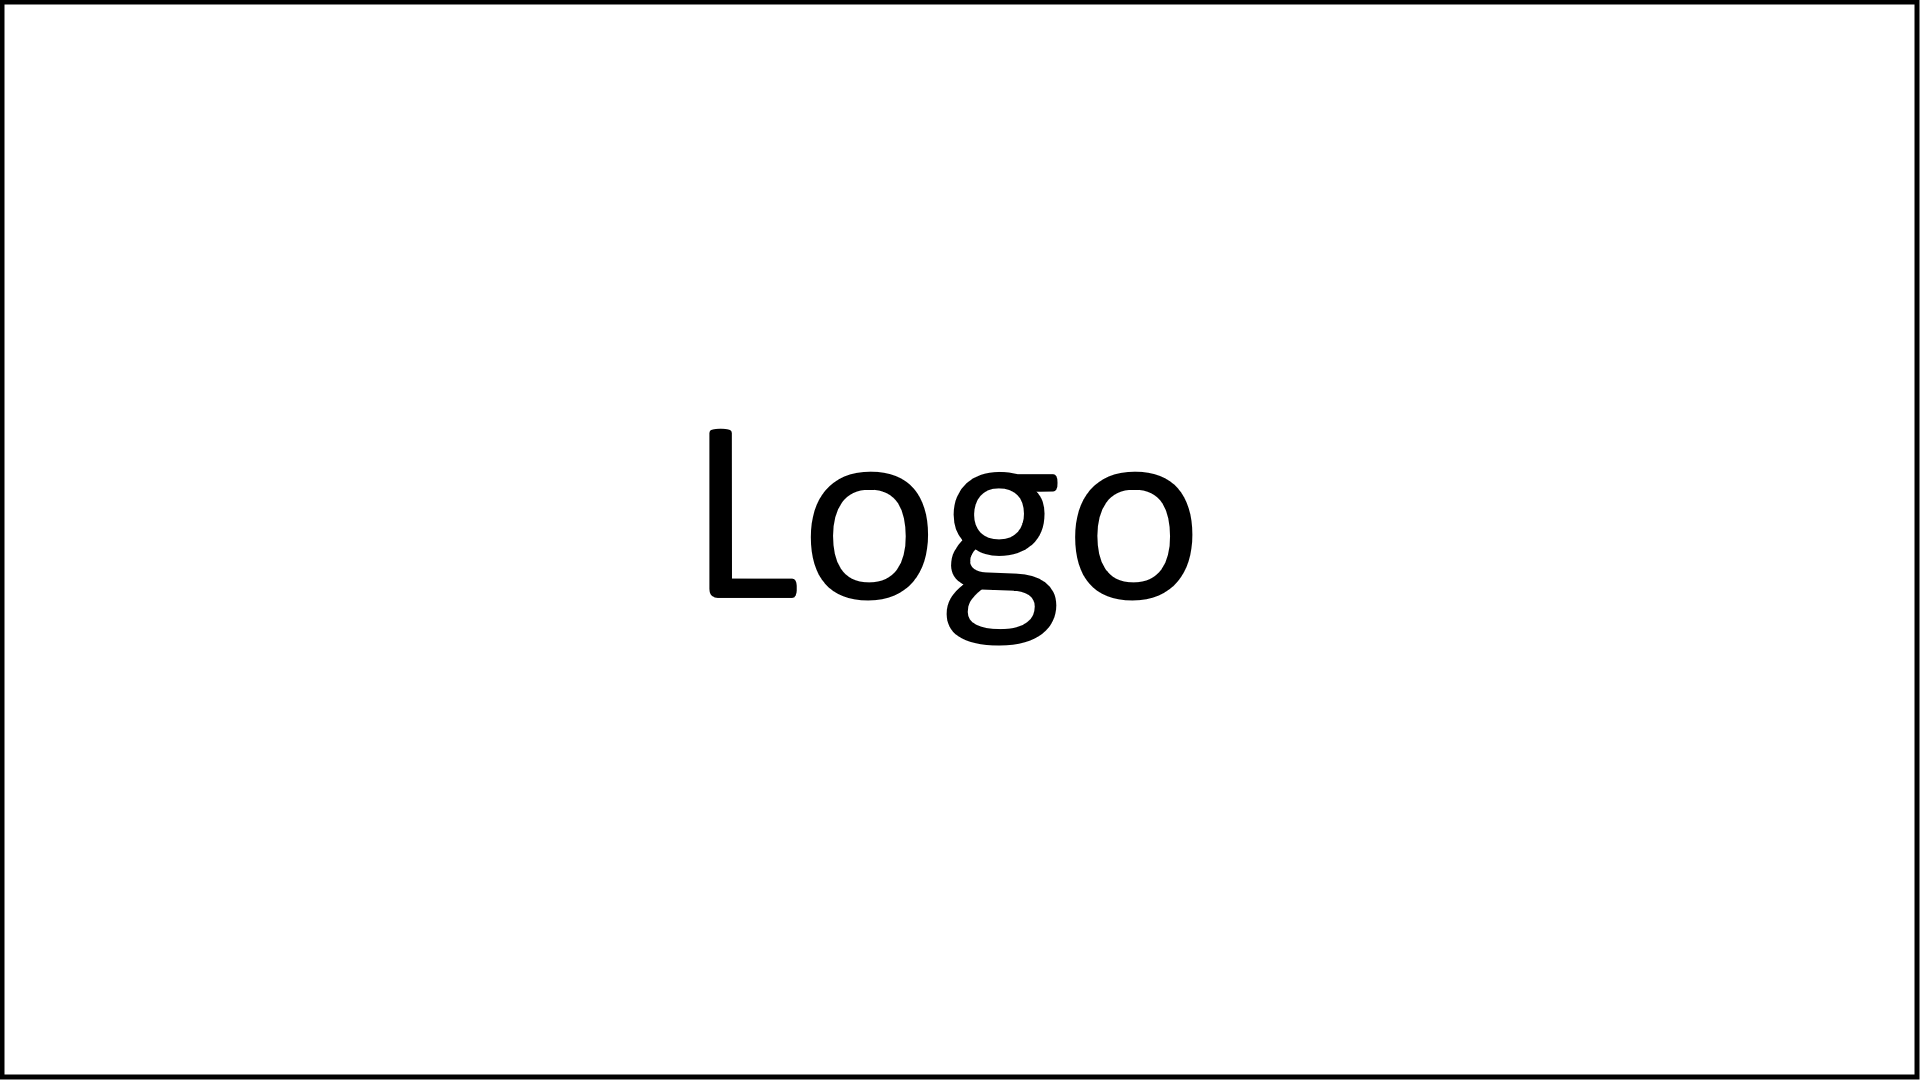
\includegraphics[width=\textwidth]{img/logo}
}

\author{
	\begin{tabular}{r l@{\hspace{8\tabcolsep}} r} 
		Eddy & Wu & \multirow{8}{*}{ 
\includegraphics{img/se-logo} } \\
		Julius & Daum \\
		Lea Marie & Sch\"umann \\
		Luca Anthony & Schwarz \\
		Natalie & Kaufhold \\
		Philipp & Wieck \\
		Till & Kurzenberger \\
		Yilmaz Atakan & Kara \\
	\end{tabular}
}

\date{\today}





% Dokument

\begin{document}
	\maketitle
	
	%%%% Bitte löschen oder auskommentieren %%%%
	%%%%%%%%% Dient nur als Hilfe %%%%%%%%%%
	
%	\chapter*{Tipps und Hilfen}\label{chp:tipps}
%	\vspace*{-1cm}
%	\begin{tcolorbox}
%		\textbf{Information:} Dieses Kapitel und alle folgenden grauen Boxen dienen als Hilfestellungen und sollen im fertigen Dokument nicht enthalten sein. 
%		%
%		\\\\
%		%
%		Zur Versionsverwaltung während des Softwareprojekts muss \textit{Git} genutzt werden.
%		Git führt Textdokumente mit unterschiedlichen Zeilenbearbeitungen automatisch zusammen.
%		Wir empfehlen den Einsatz von \LaTeX~für alle Textdokumente.
%		Um das Auto-Merging zu unterstützen, sollte nach jedem Satzende eine neue Zeile im Quelltext begonnen werden.
%		Die .tex-Datei dieser PDF verdeutlicht dies.
%		Erkennt Git, dass eine gleiche Zeile bearbeitet wurde, wird ein Konflikt auftreten.
%		Dieser kann in der entsprechenden Datei von Hand mittels eines Texteditors behoben werden.
%		%
%		\\\\
%		%
%		Fußnoten\footnote{\url{https://www.se.informatik.uni-kiel.de/en}} werden für Homepages genutzt.
%		Zitierungen können mittels eines \textit{cite}-Befehls gesetzt, z.B. \textit{citep}~\citep{Shaw2003WritingGoodSoftwareEngineeringesearchPapersMinitutorial}.
%		%
%		\\\\
%		%
%		Tipps zur UML-Modellierung können im SE-Wiki\footnote{\url{https://git.informatik.uni-kiel.de/ag-se/teaching-public/wikis/home}} nachgelesen werden.
%		Achtet darauf, dass eure Diagramme stets lesbar (Vektor-Grafiken!) und gut strukturiert sind.
%		Oftmals ist es sinnvoll ein bis zwei Sätze zusätzlich für Diagrammelemente zu formulieren.
%		So können Missverständnisse ausgeschlossen werden, was einen Einfluss auf die Korrektur haben kann.
%		Diagramme für unwichtige Tätigkeiten (z.B. Login / Logout, User erstellen / löschen, Passwort ändern etc.) sind nicht erforderlich.	
%	\end{tcolorbox}
%	
%	\todo[inline]{So kann eine TODO-Notiz erzeugt werden}
%	
%	\begin{figure}[h]
%		\centering
%		\missingfigure{So kann eine Placeholder-Grafik beispielsweise in den Text eingefügt werden.}		
%		\caption{Beschreibung}
%		\label{fig:x}
%	\end{figure}
		
	%%%%%%%%%%%%%%%%%%%%%%%%%%%%%%
	
	\tableofcontents
	
	\chapter{Lizenz}\label{chp:lizenz}
	\pagenumbering{arabic} % Nummerierung starten
	\begin{tcolorbox}
Die Abgabe der Software und des Pflichtenhefts muss eine genaue Angabe der Lizenz enthalten, unter der die zu entwickelnde Software lizensiert wird.
Um eine spätere Weiterverwendung und einen Praxiseinsatz der Software zu ermöglichen, empfehlen wir die Apache Lizenz 2.0~\footnote{\url{http://www.apache.org/licenses/LICENSE-2.0}}.
In diesem Kapitel soll die verwendete Lizenz notiert werden.
\end{tcolorbox}
	
	\chapter{Zielbestimmungen}\label{chp:zielbestimmungen}
	%\begin{tcolorbox}
%Die Zielbestimmungen dienen dazu, die Ziele der Anforderungen nach Priorität zu sortieren. 
%Es wird zwischen \textit{Muss}-, \textit{Soll-}, \textit{Kann-} und \textit{Abgrenzungskriterien} unterschieden, wobei weitere Einteilungen (z.B. nach Gerät oder Benutzer) innerhalb der Kategorien möglich sind.
%%
%\\\\
%%
%Die \textit{Musskriterien} umfassen alle Ziele und Funktionalitäten, die für einen Einsatz des entwickelten Produktes unabdingbar sind.
%Sie müssen daher ohne Kompromisse implementiert werden.
%Ein Wegfall eines einzelnen Musskriteriums würde das Produkt außer Betrieb setzen.
%%
%\\\\
%%
%\textit{Sollkriterien} (auch Wunschkriterien genannt) sind gewünschte Funktionen, die ebenfalls implementiert werden müssen, deren Wegfall auf Grund von unüblichen Umständen aber nicht den Einsatz des Produkts hindern würde.
%%
%\\\\
%%
%Die \textit{Kannkriterien} sind alle Ziele, die wünschenswert sind, aber nicht zwingend notwendige Funktionen darstellen. 
%Oftmals werden diese nach Beendigung der höher priorisierten Kriterien umgesetzt.
%%
%\\\\
%%
%\textit{Abgrenzungskriterien} dienen dazu die Grenzen des Produkts zu definieren.
%Es soll erkennbar sein, was explizit \textbf{nicht} umgesetzt wird, damit Kunden nichts Falsches erwarten und Ziele stets klar definiert bleiben.
%%
%\\\\
%%
%Für die Auflistung der Zielbestimmungen können Fließtexte oder auch Auflistungen mit ganzen Sätzen genutzt werden. 
%\end{tcolorbox}

\textbf{Musskriterien}:
\begin{itemize}
	\item Es muss ein Accountmanagement vorhanden sein, welches verschiedene Rollen unterstützt.
	\item Die Software muss dazu in der Lage sein, Vertragsdaten zu übernehmen.
	\item Die Software muss den Baufortschritt sowie Leistungspositionen anzeigen können.
	\item Sowohl Website als auch App müssen eine graphische Nutzeroberfläche anbieten.
	\item Die App muss den Status von Leistungspositionen anzeigen können.
	Diese müssen innerhalb der App auch verändert werden können.
\end{itemize}

\noindent \textbf{Sollkriterien}:
\begin{itemize}
	\item Die Website soll folgende Diagramme darstellen können:
		\begin{itemize}
		\item Diagramme über den Baufortschritt eines Projektes
		\item Diagramme über die Zustände der Leistungspositionen aus einem oder mehreren Verträgen
		\end{itemize}
	\item Die Nutzeroberflächen von Desktop-Website und App sollen übersichtlich, gut bedienbar und insgesamt benutzerfreundlich sein.
	\item Die App soll die Möglichkeit anbieten, den Baufortschritt eines Projektes mittels Fotos zu dokumentieren.
	Des Weiteren soll die App offline verwendbar sein, insbesondere soll somit die Fotodokumentation auch offline möglich sein.
\end{itemize}

\noindent \textbf{Kannkriterien}:
\begin{itemize}
	\item Die Website kann eine mobile Version der Nutzeroberfläche anzeigen.
	\item Die Fotos zur Dokumentation des Baufortschritts können von anderen Mitarbeitern auf korrekte Durchführung überprüft werden.
	So ist es auch möglich, Kommentare zu Fotos abzugeben und Produktmängel zu melden.
	\item Die Website kann diverse Möglichkeiten anbieten, nach denen Diagramme gefiltert werden können.
	\item Die Website kann Nutzern die Möglichkeit anbieten, aus Leistungspositionen, Verträgen und Projekten eigene Diagramme zu erstellen.
\end{itemize}

\noindent \textbf{Abgrenzungskriterien}:
\begin{itemize}
	\item Es wird keine iOS-Version der App geben.
	\item Fotos werden nicht mittels Machine Learning von der Software ausgewertet.
	\item Es wird keine Kompatibilität der Website für veraltete Browserversionen garantiert.
	\item Es wird keine Kompatibilität der App für Androidversionen vor Android 6 garantiert.
\end{itemize}
	
	\chapter{Produkteinsatz}\label{chp:produkteinsatz}
	\begin{tcolorbox}
In diesem Kapitel werden die folgenden drei Punkte erläutert:
\begin{enumerate}
	\item \textit{Anwendungsgebiete:} Was ist der Zweck des Produkts?
	\item \textit{Zielgruppen:} Für welche Benutzer (oder auch Rollen) ist das Produkt bestimmt?
	Welche Qualifikationen brauchen die Personen?
\end{enumerate}

\noindent Die einzelnen Teile des Produkteinsatzes werden üblicherweise als Fließtexte geschrieben.
\end{tcolorbox}


	\chapter{Produktfunktionen}\label{chp:produktfunktionen}
	\begin{tcolorbox}
Die Produktfunktionen beschreiben jede einzelne Funktion des Produkts mittels Anwendungsfalldiagrammen und Anwendungsfalltabellen.
Diese sollen möglichst ausschlaggebend für das zu entwickelnde System sein und nicht simple Produktfunktionen wie z.B. Login, Account erstellen, Gruppe beitreten, Passwort ändern oder ähnliches zeigen.
\autoref{fig:anwendungsfall-app-tabelle-xx-1} stellt eine exemplarische Tabelle für die Beschreibung eines Anwendungsfalls dar. Stil und Formatierung sind variabel. Nicht jede Zelle muss immer gefüllt sein.
\\\\
In  Tabelle~\autoref{fig:akteur-tabelle} werden alle auftretenden Akteure beschrieben.


\end{tcolorbox}

\begin{figure}[h]
	\centering
	
	\begin{tabularx}{\textwidth}{ p{.2\textwidth} | p{.2\textwidth} | X }
		\textbf{Akteur} & \textbf{Beschreibung} & \textbf{Verwendet in Anwendungsfall} \\ \hline
		Informatiker & Programmiert tolle Sachen & Programmieren, Kaffee trinken, Schlafen
	\end{tabularx}
	
	\caption{Beschreibung der Akteure}
	\label{fig:akteur-tabelle}
\end{figure}

\newpage

\section{Anwendungsfalldiagramm - App}

\begin{figure}[h]
	\centering
    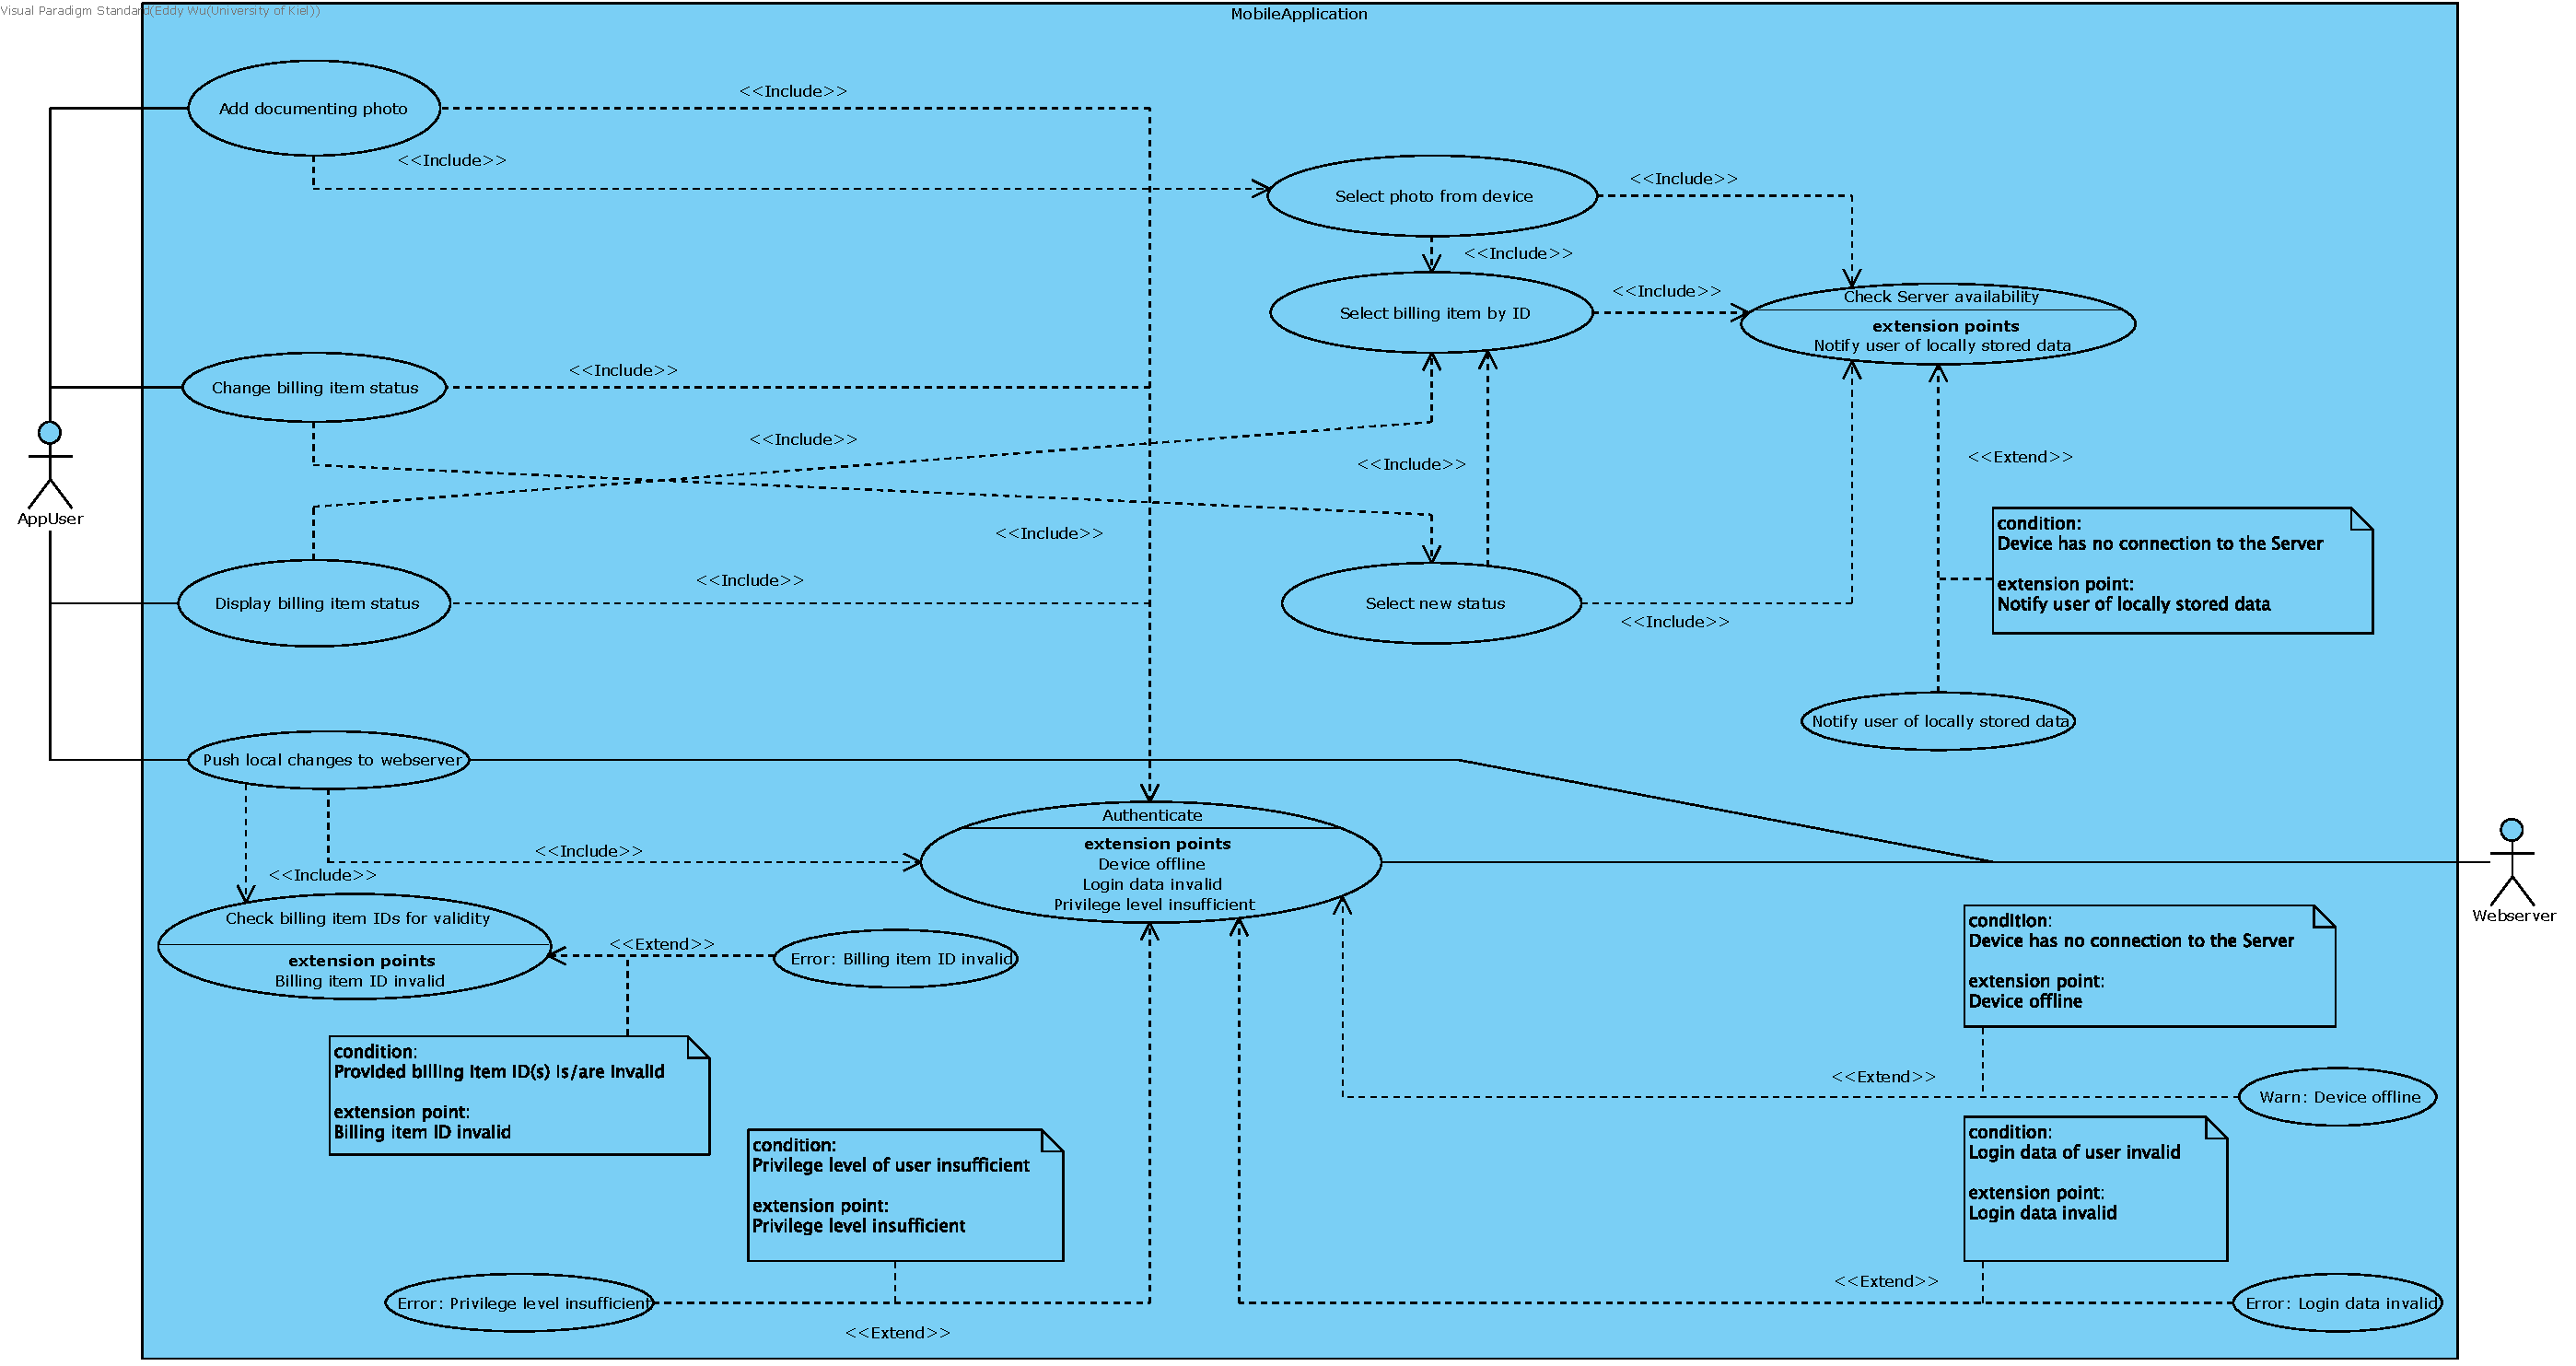
\includegraphics[width=\linewidth]{img/diagrams/Mobile_Application.pdf}
     %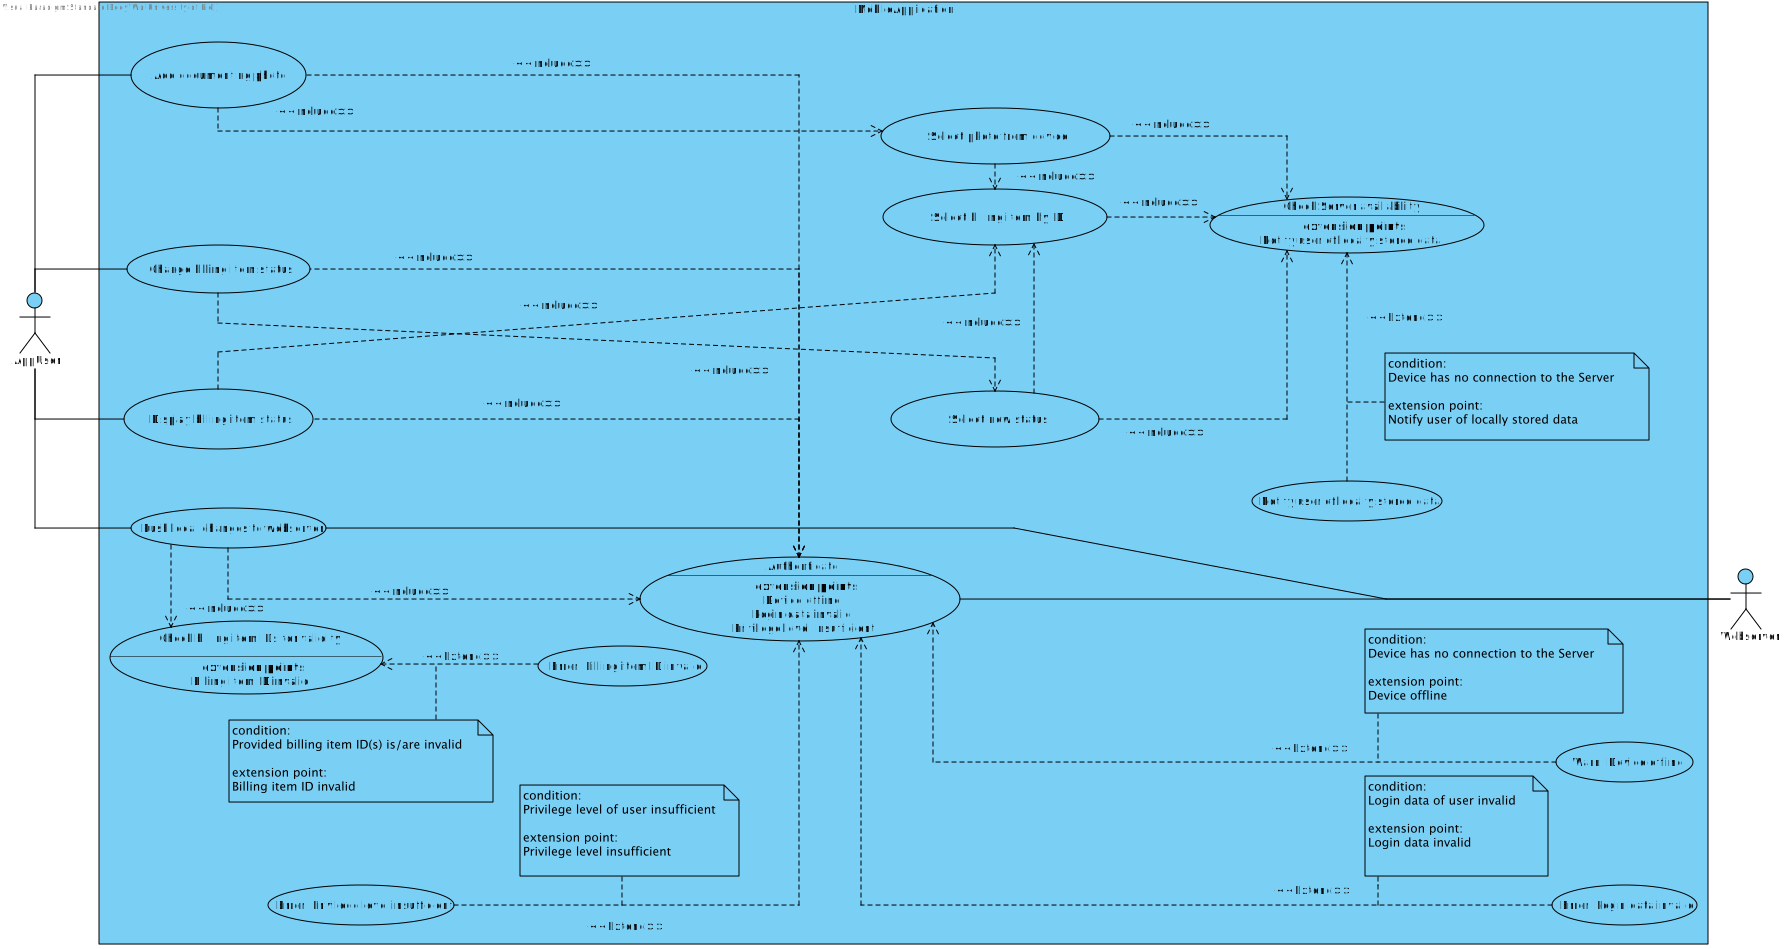
\includegraphics[width=\linewidth]{img/diagrams/Mobile_Application.svg}
     %\includesvg{img/diagrams/Mobile_Application.svg}
	\caption{Anwendungsfalldiagramm - App}
	\label{fig:anwendungsfalldiagramm-app}
\end{figure}

\newpage

\begin{figure}[h]
	\centering
	\begin{tabularx}{\textwidth}{ X | X }
		\textbf{Anwendungsfall ID} & APP-1 \\ \hline
		\textbf{Anwendungsfallname} & Push local changes to webserver\\ \hline
		\textbf{Initiierender Akteur} & Nutzer der App \\ \hline
		\textbf{Weitere Akteure} & Webserver  \\ \hline
		\textbf{Kurzbeschreibung} & Der Benutzer der Applikation kann lokale \"Anderungen,  bspw. \"Anderungen zum Baustatus einzelner Leistungspositionen oder Fotos mit Kommentar von der Baustelle,  an den Webserver schicken.  Diese \"Anderungen und Fotos mit Kommentar k\"onnen dann enstprechend  \"uber die Webanwendung eingesehen werden.  \\ \hline
		\textbf{Vorbedingungen} & Der AppUser ist registriert und entsprechend eingeloggt \\ \hline
		\textbf{Nachbedingungen} & Die lokalen Daten wurden an den Webserver geschickt\\ \hline
		\textbf{Ablauf} &
			\begin{enumerate}
				\item Der AppUser hat den Status einer Leistungspositionen  lokal ge\"andert.
				\item Der Benutzer verwendet die Funktion der App,  um seine lokale \"Anderung an den Webserver zu \"ubertragen.
				\item Es besteht eine Internetverbindung und der AppUser erh\"alt die R\"uckmeldung,  dass das Vorhaben erfolgreich ausgef\"uhrt wurde.  
				\item Die \"Anderung befindet sich nun auf dem Webserver.
			\end{enumerate}
			\end{tabularx}
	\caption{Anwendungsfall APP-1}
	\label{fig:anwendungsfall-app-tabelle-APP-1-1}
\end{figure}
			\begin{figure}[h]
	\centering
	\begin{tabularx}{\textwidth}{ X | X }
		\textbf{Alternative} & 
				\begin{enumerate}
					 \item Der AppUser hat seinen Benutzerrechten entsprechend ein Foto zur Dokumentation einer Leistungsposition angefertigt.
					 \item Das Foto soll nun durch Bet\"atigen der entsprechenden Funktion der mobilen Applikation auf den Webserver hochgeladen werden.
					 \item Es besteht eine Internetverbindung und der AppUser erh\"alt eine entsprechende Meldung,  dass der Upload erfolgt.
					 \item Das Foto wird an den Webserver \"ubertragen.
				\end{enumerate}  \\ \hline
						\textbf{Ausnahme} &
				\begin{enumerate}
					 \item Der AppUser m\"ochte eine \"Anderung an dem Status einer Leistungsposition oder ein Foto zur Dokumentation mit Kommentar an den Webserver \"ubertragen und verwendet die enstprechende Funktionalit\"at der Applikation.
					 \item Der User erh\"alt eine Fehlermeldung, da seine Rechte nicht ausreichen um diese Aktion durchzuf\"uhren.
					 \item Die \"Anderungen am Status der Leistungsposition und/oder das Foto mit Kommentar werden nicht an den Webserver \"ubertragen.
					 \end{enumerate} \\ \hline
	\end{tabularx}
	\caption{Anwendungsfall APP-1}
	\label{fig:anwendungsfall-app-tabelle-APP-1-2}
\end{figure}
			\begin{figure}[h]
	\centering
	\begin{tabularx}{\textwidth}{ X | X }
					 	\textbf{Ausnahme} &
				\begin{enumerate}
					\item Die lokalen \"Anderungen durch den Benutzer sollen durch Bet\"atigung der entsprechenden Funktion in der App an den Webserver \"ubertragen werden.
					\item Der AppUser erh\"alt eine Fehlermeldung,  da zur Zeit f\"ur das verwendetete Ger\"at keine (ausreichende) Internetverbindung besteht. 
					\item Der Benutzer erh\"alt eine R\"uckmeldung,  dass zur Zeit keine Internetverbindung besteht und lokale \"Anderungen zwischengespeichert werden.
					\item Sobald eine ausreichende Internetverbindung besteht,  werden die entsprechenden Daten an den Webserver \"ubertragen.
				\end{enumerate} 
				 	\end{tabularx}
	\caption{Anwendungsfall APP-1}
	\label{fig:anwendungsfall-app-tabelle-APP-1-3}
\end{figure}
			\begin{figure}[h]
	\centering
	\begin{tabularx}{\textwidth}{ X | X }
		\textbf{Ausnahme} &
				\begin{enumerate}
				\item Der Benutzer loggt sich innerhalb der App mit seinen registrierten Benutzerdaten, bestehend aus Benutzername und Passwort,  ein.  
					 \item Der AppUser m\"ochte eine \"Anderung an dem Status einer Leistungsposition an den Webserver \"ubertragen und verwendet die entsprechende Funktion in der Applikation. 
					 \item Die Identifikationsnummer der betroffenen Leistungsposition ist nicht g\"ultig.
					 \item Der User erh\"alt eine Fehlermeldung.
					 \item Die \"Anderungen am Status der Leistungsposition werden nicht an den Webserver \"ubertragen.
				\end{enumerate} \\ \hline
						\textbf{Ausnahme} &
				\begin{enumerate}
					 \item Der AppUser m\"ochte eine lokale \"Anderung an dem Status einer Leistungsposition oder ein Foto mit Kommentar an den Webserver \"ubertragen und verwendet die entsprechende Funktion in der Applikation. 
					 \item Die Identifikationsnummer der betroffenen Leistungsposition ist nicht g\"ultig.
					 \item Der User erh\"alt eine Fehlermeldung.
					 \item Die \"Anderungen am Status der Leistungsposition oder das Foto mit Kommentar werden nicht an den Webserver \"ubertragen.
				\end{enumerate} \\ \hline
		\textbf{Benutzte Anwendungsfälle} & Benutzerverwaltung (ACC-1) \\ \hline
		\textbf{Spezielle Anforderungen} & - \\ \hline
		\textbf{Annahmen} & -
	\end{tabularx}
	\caption{Anwendungsfall APP-1}
	\label{fig:anwendungsfall-app-tabelle-APP-1-4}
\end{figure}

\clearpage

\section{Anwendungsfalldiagramme - Webserver}

\subsection{Account-Management}

\begin{figure}[h]
	\centering
	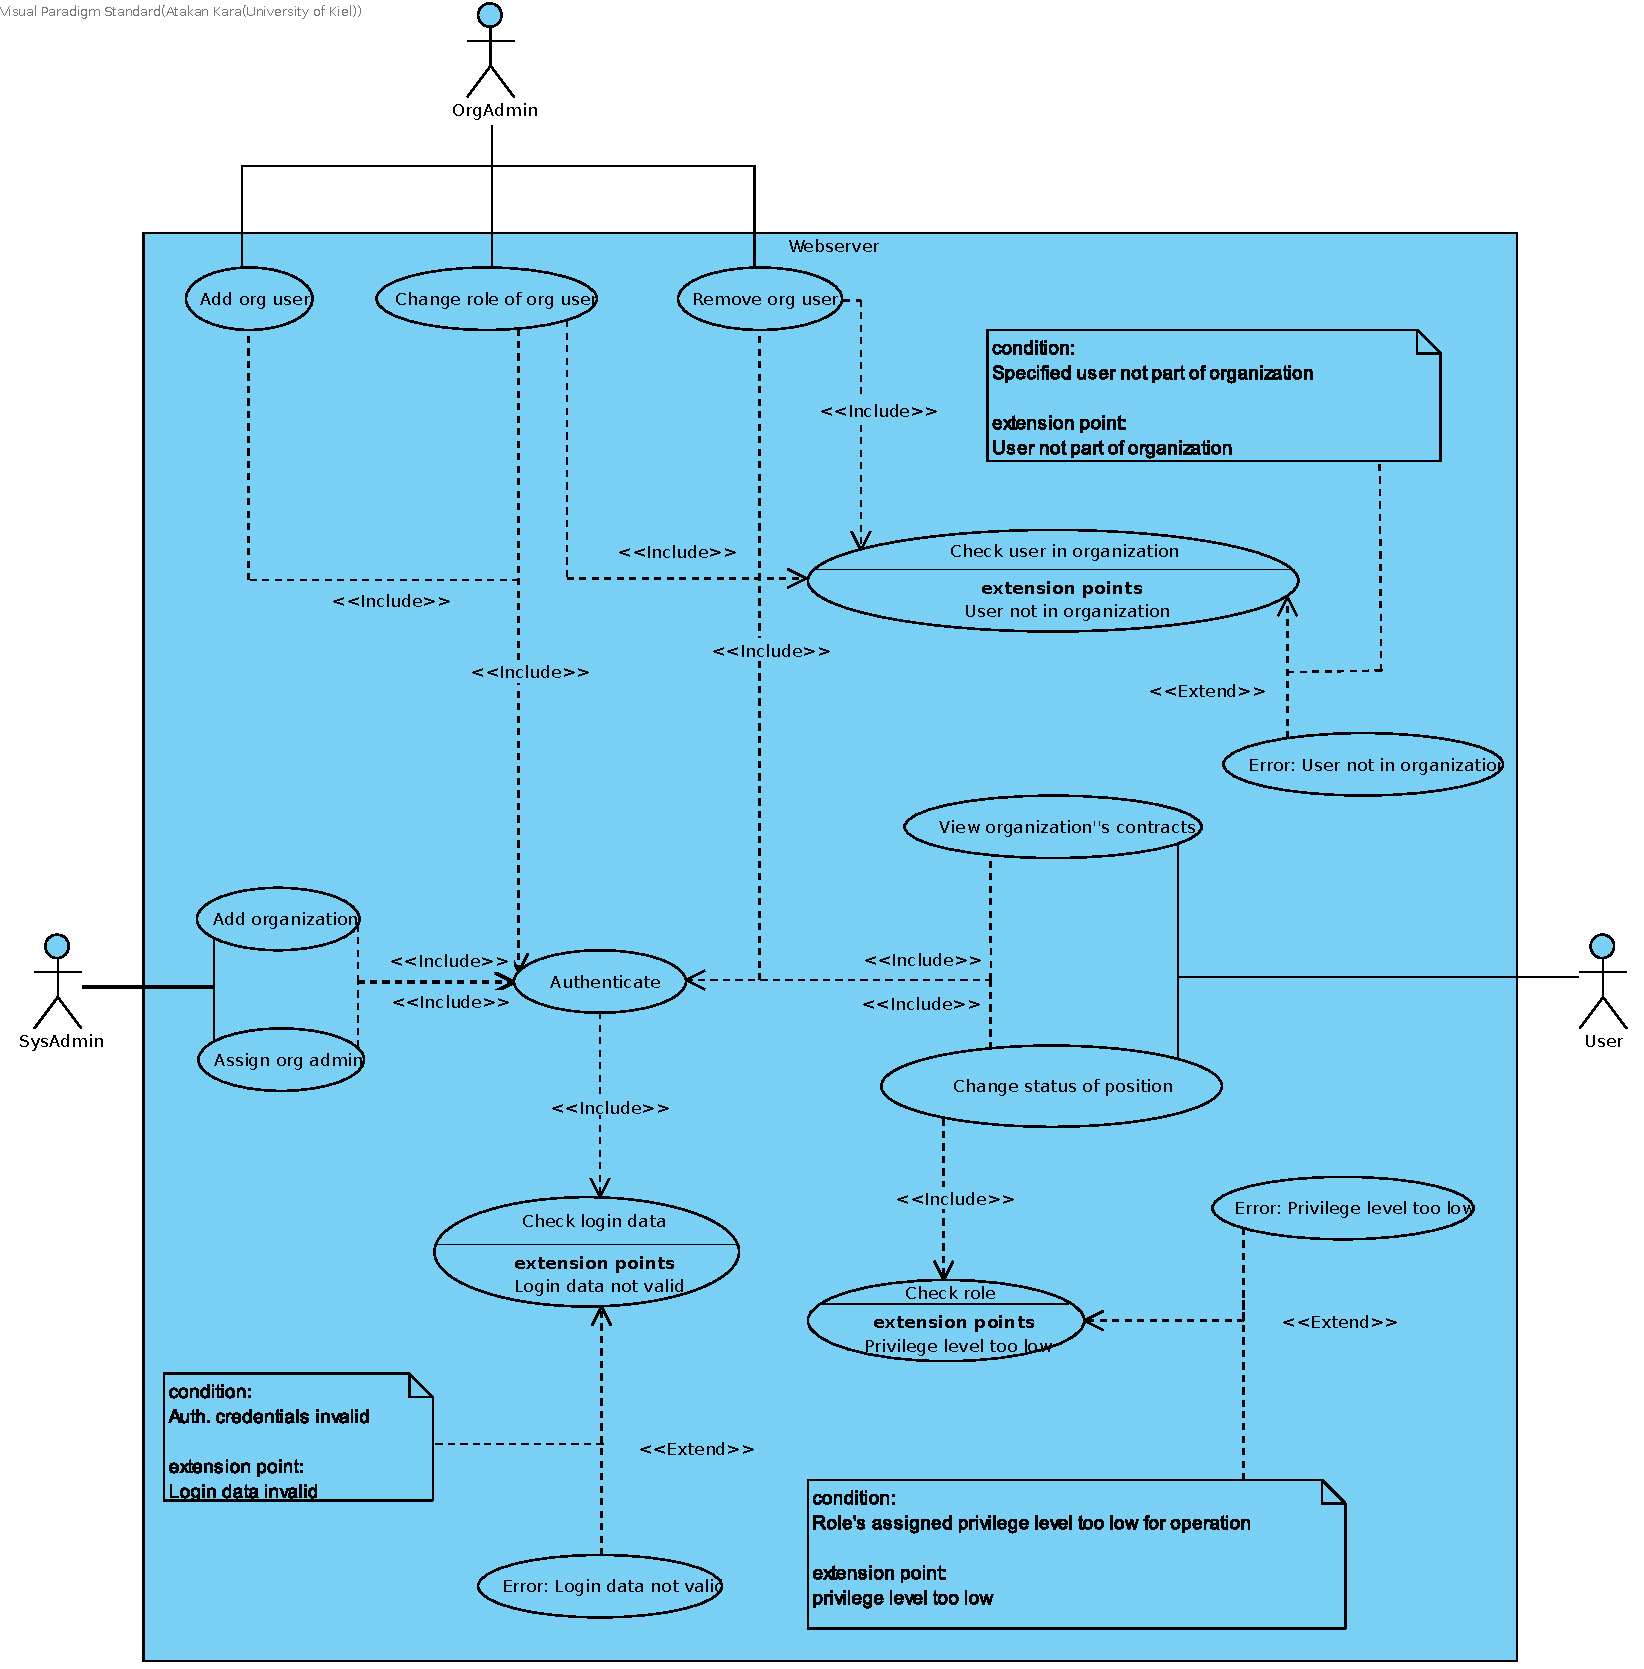
\includegraphics[width=\linewidth]{img/diagrams/Acc_Management_Web.pdf}
	%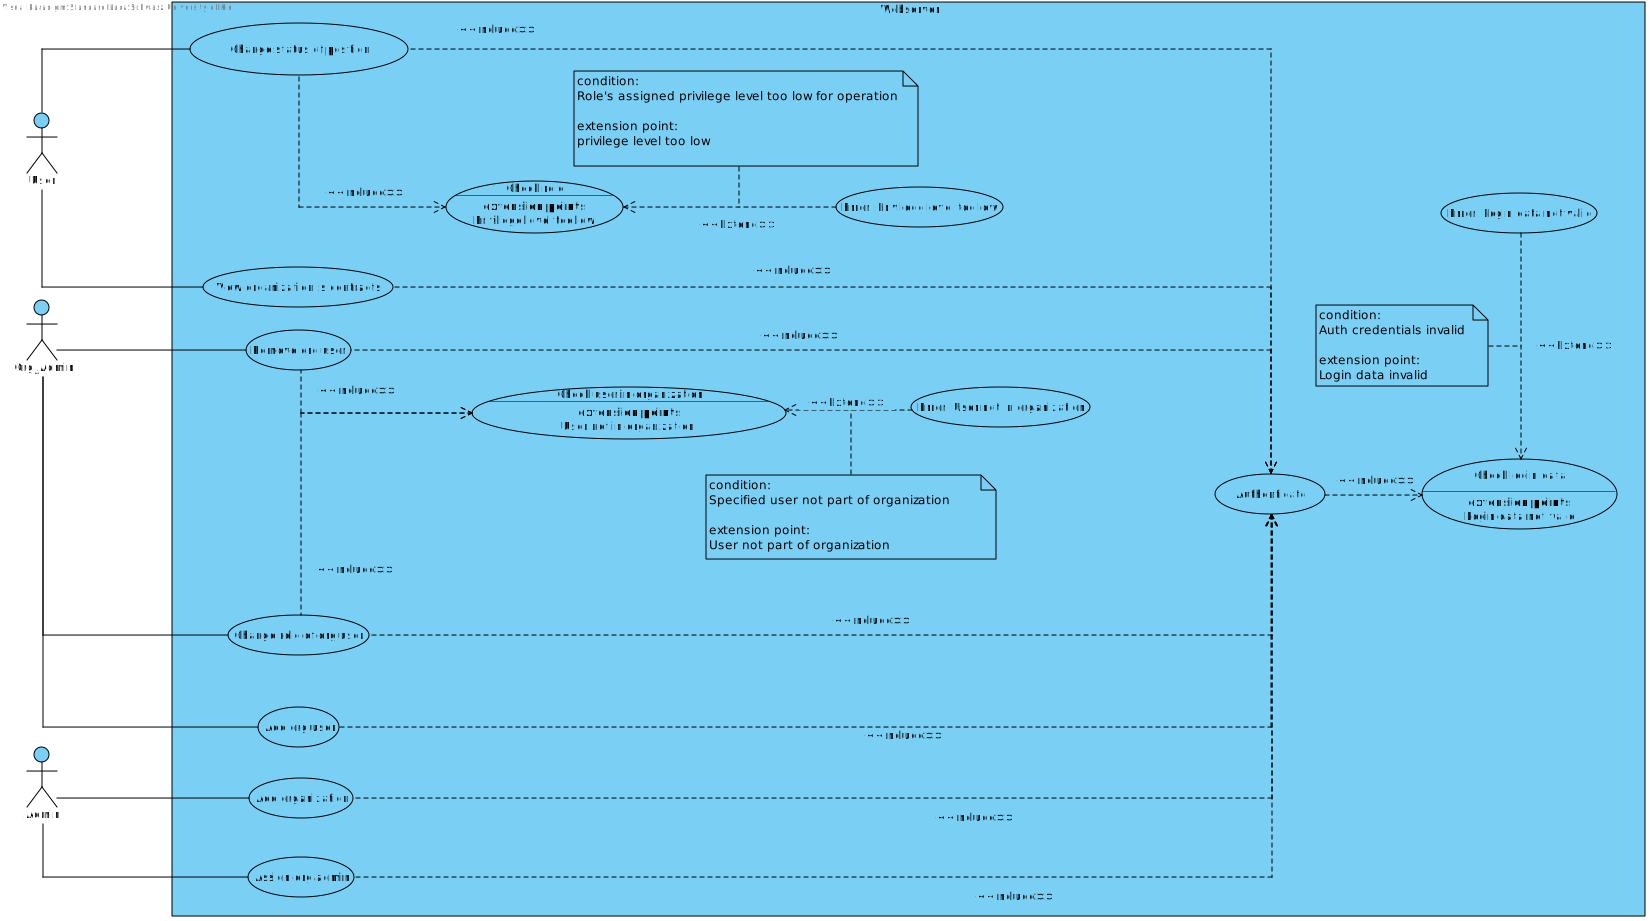
\includegraphics[width=\linewidth]{img/diagrams/Acc_Management_Web.svg}
	\caption{Anwendungsfalldiagramm - Account-Management Webserver}
	\label{fig:anwendungsfalldiagramm-acc}
\end{figure}

\newpage

\begin{figure}[h]
	\centering
	\begin{tabularx}{\textwidth}{ X | X }
		\textbf{Anwendungsfall ID} & ACC-1 \\ \hline
		%\textbf{Anwendungsfallname} & Change status of position\\ \hline
		\textbf{Anwendungsfallname} & Modifizieren des Status einer Leistungsposition \\ \hline
		\textbf{Initiierender Akteur} & Nutzer \\ \hline
		\textbf{Weitere Akteure} & -  \\ \hline
		\textbf{Kurzbeschreibung} & Der User kann den Status von Leistungspositionen ver\"andern \\ \hline
		\textbf{Vorbedingungen} & User ist entsprechend eingeloggt, Rechte des Users sind ausreichend f\"ur diese Operation \\ \hline
		\textbf{Nachbedingungen} & Status wurde ver\"andert \\ \hline
		\textbf{Ablauf} &
		\begin{enumerate}
			\item Der User \"andert den Status einer Leistungsposition und w\"ahlt die entsprechende Funktion der Weboberfl\"ache, dass diese \"Anderung \"ubernommen werden sollen.
			\item Die Aktion war erfolgreich und die \"Anderung wurde \"ubernommen.  Der User erh\"alt eine R\"uckmeldung \"uber den Erfolg der Aktion.
		\end{enumerate} \\ \hline
		\textbf{Alternative} & -
		\\ \hline
		\textbf{Ausnahme} &
		\begin{enumerate}
			\item Der User \"andert den Status einer Leistungsposition und w\"ahlt die entsprechende Funktion der Weboberfl\"ache,  dass diese \"Anderung \"ubernommen werden sollen.
			\item Der User verf\"ugt nicht \"uber die entsprechenden Rechte die Aktion durchzuf\"uhren und erh\"alt eine Fehlermeldung. Der bisherige Status der Leistungsposition bleibt bestehen.
		\end{enumerate}  \\ \hline
		\textbf{Benutzte Anwendungsfälle} & Benutzerverwaltung (ACC-1) \\ \hline
		\textbf{Spezielle Anforderungen} & - \\ \hline
		\textbf{Annahmen} & -
	\end{tabularx}
	\caption{Anwendungsfall ACC-1}
	\label{fig:anwendungsfall-server-tabelle-ACC-1}
\end{figure}

\clearpage

\subsection{Diagrammdarstellung}

\begin{figure}[h]
	\centering
	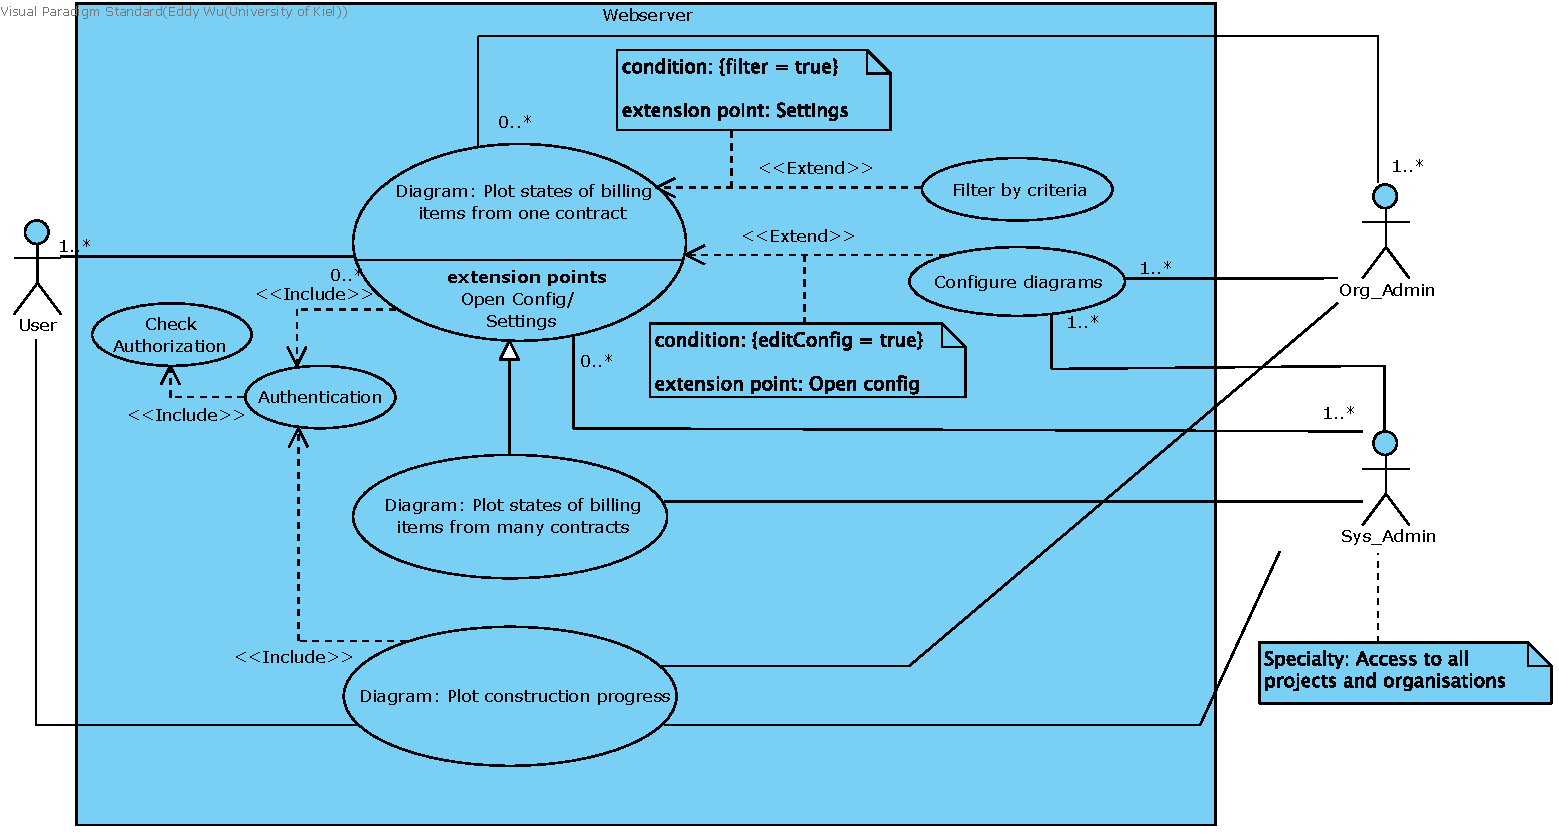
\includegraphics[width=\linewidth]{img/diagrams/Diagram_Display_Management_Web.pdf}
	%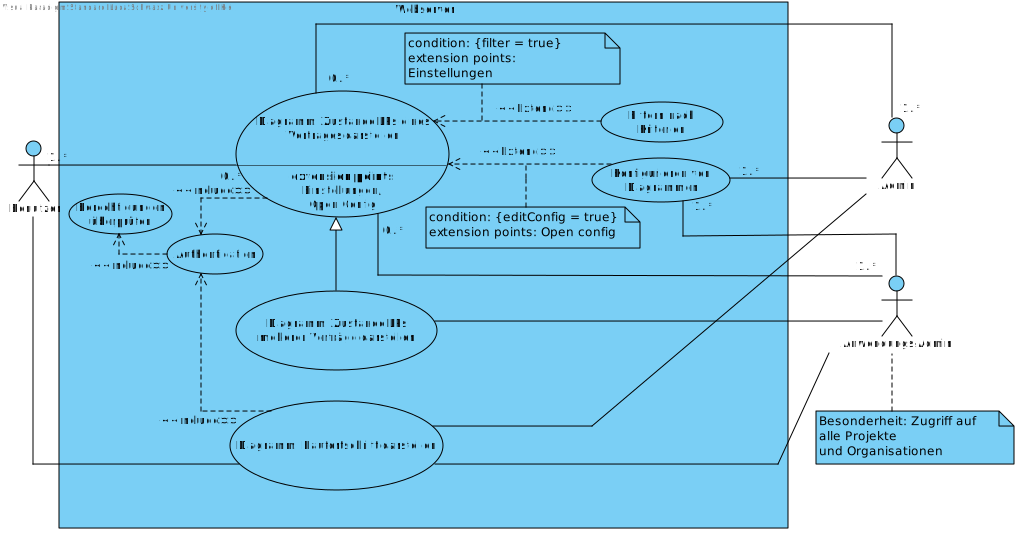
\includegraphics[width=\linewidth]{img/diagrams/Diagram_Display_Management_Web.svg}
	\caption{Anwendungsfalldiagramm - Diagrammdarstellung}
	\label{fig:anwendungsfalldiagramm-dia-verwaltung}
\end{figure}

\newpage

\begin{figure}[h]
	\centering
	\begin{tabularx}{\textwidth}{ X | X }
		\textbf{Anwendungsfall ID} & DIA-1 \\ \hline
		\textbf{Anwendungsfallname} & Diagrammdarstellung \\ \hline
		\textbf{Initiierender Akteur} & Systemadministrator \\ \hline
		\textbf{Weitere Akteure} & Organisationsadministrator, Mitarbeiter \\ \hline
		\textbf{Kurzbeschreibung} & Darstellung und mögliche Filterung der vom Server automatisch erzeugten Diagramme innerhalb der Webapplikation.  \\ \hline
		\textbf{Vorbedingungen} & Funktionierende Internetverbindung, bestätigte Berechtigungen (Authentifiziert)  \\ \hline
		\textbf{Nachbedingungen} &  -  \\ \hline
		\textbf{Ablauf} &
		\begin{enumerate}
			%\item Erfolgreich authentifizieren (passende Rolle).
			\item Authentifizieren (passende Rolle).
			\item Der Nutzer wechselt in den Reiter der Diagramme.
			%\item Darstellen eines allgemeinen (alle Leistungspunkte umfassend) Diagramms zu einem oder mehreren Verträgen.
			\item Der Nutzer wählt ein alle Leistungspunkte umfassendes Diagramm eines oder mehrere Verträge zur Darstellung.
			\item Das Diagramm wird angezeigt.
		\end{enumerate} \\ \hline
		\multirow{2}{*}{\textbf{Alternativen}} &
		%%\textbf{Alternative} &
		\begin{enumerate}
			%\item Erfolgreich authentifizieren (passende Rolle).
			\item Authentifizieren (passende Rolle).
			\item Der Nutzer wechselt in den Reiter der Diagramme.
			\item Der Nutzer filtert nach bestimmten Kriterien.
			%\item Darstellen eines Diagramms zu einem oder mehreren Verträgen.
			\item Das Diagramm wird angezeigt.
		\end{enumerate} \\\cline{2-2} &
		\begin{enumerate}
			%\item Erfolgreich authentifizieren (passende Rolle).
			\item Authentifizieren (passende Rolle).
			\item Der Nutzer wechselt in den Reiter der Diagramme.
			\item Der Nutzer wählt das Diagramm zum Baufortschritt eines Projektes.
			\item Das Diagramm wird angezeigt.
		\end{enumerate}  \\ \hline
		\end{tabularx}
	\caption{Anwendungsfall DIA-1}
	\label{fig:anwendungsfall-diagrammdarstellung-tabelle-DIA-1}
\end{figure}

\newpage

\begin{figure}[h]
	\centering
	\begin{tabularx}{\textwidth}{ X | X }		
		%%\textbf{Ausnahme} &
		\multirow{2}{*}{\textbf{Ausnahme}} &
		\begin{enumerate} % Projekt/Vertrag nicht vorhanden.
			%\item Erfolgreich authentifizieren (passende Rolle).
			\item Authentifizieren (passende Rolle).
			\item Der Nutzer wechselt in den Reiter der Diagramme.
			\item Der Nutzer wählt ein nicht-existentes Projekt aus.
			\item Fehlermeldung!
		\end{enumerate} \\\cline{2-2} &
		\begin{enumerate} % Kriterien werden nicht erfüllt.
			\item Authentifizieren (passende Rolle).
			\item Der Nutzer wechselt in den Reiter der Diagramme.
			\item Der Nutzer filtert nach bestimmten Kriterien.
			\item Die Kriterien werden von keinem Diagramm erfüllt.
			\item Fehlermeldung!
		\end{enumerate}  \\\cline{2-2} &
		\begin{enumerate} % Fehlende Berechtigungen.
			%\item Erfolgreich authentifizieren (\textbf{keine} passende Rolle).
			\item Authentifizieren (\textbf{keine} passende Rolle).
			\item Der Nutzer wechselt in den Reiter der Diagramme.
			%\item Diagramm ohne passende Rolle anzeigen lassen.
			\item Der Nutzer wählt ein Diagramm, für welches er keine Rechte hat.
			\item Fehlermeldung!
		\end{enumerate}  \\\cline{2-2} &
		\begin{enumerate} % Fehlende Berechtigungen für einzelne LPs.
			%\item Erfolgreich authentifizieren (\textbf{keine} passende Rolle).
			\item Authentifizieren (\textbf{keine} passende Rolle).
			\item Der Nutzer wechselt in den Reiter der Diagramme.
			%\item Diagramm ohne passende Rolle anzeigen lassen.
			\item Der Nutzer filtert nach bestimmten Kriterien, wofür er keine Rechte hat.
			\item Fehlermeldung!
		\end{enumerate}  \\ \hline
		\textbf{Benutzte Anwendungsfälle} & Benutzerverwaltung (ACC-1) \\ \hline
		\textbf{Spezielle Anforderungen} & - \\ \hline
		\textbf{Annahmen} & -
	\end{tabularx}
	\caption{Anwendungsfall DIA-1}
	\label{fig:anwendungsfall-diagrammdarstellung-tabelle-DIA-1}
\end{figure}

%\newpage
\clearpage

\subsection{Diagrammerstellung}

\begin{figure}[h]
	\centering
	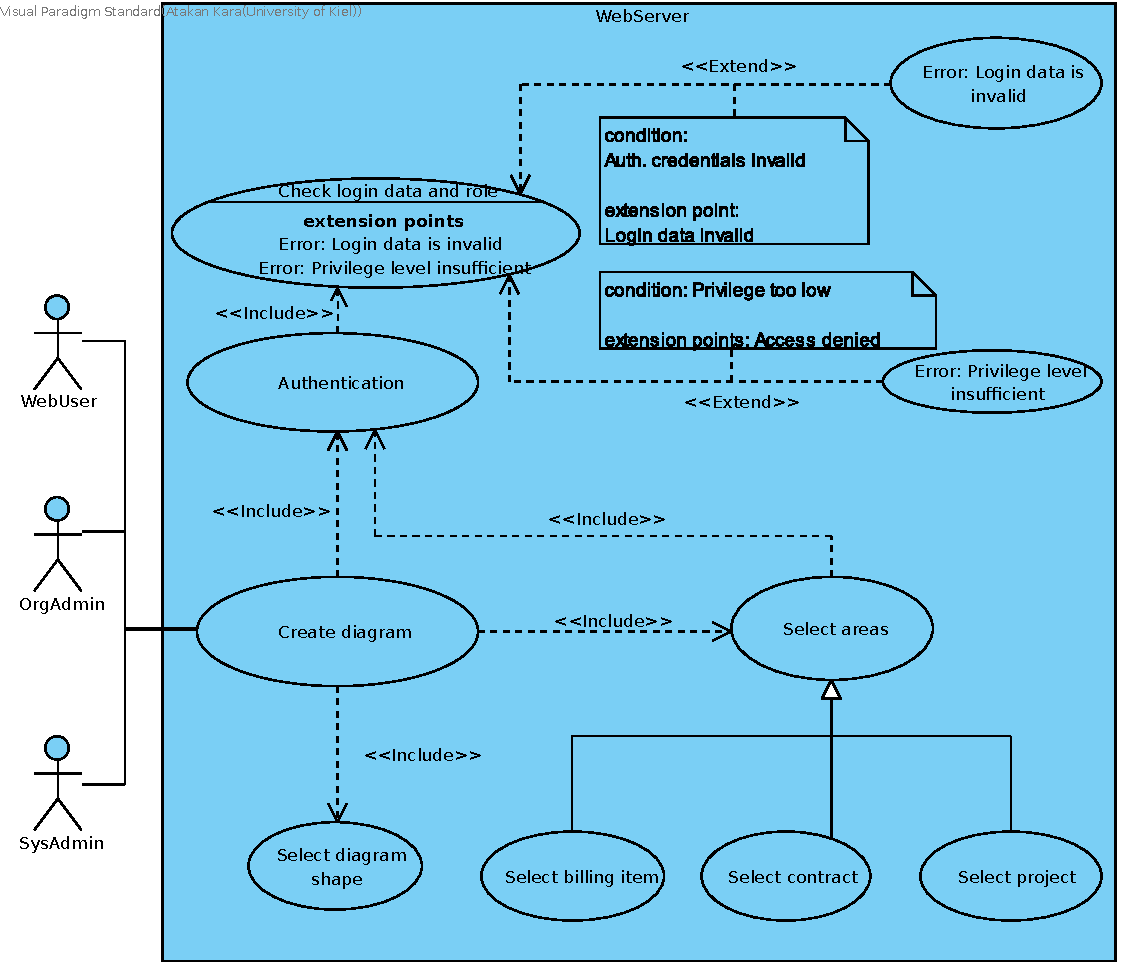
\includegraphics[width=\linewidth]{img/diagrams/Create_Custom_Diagram.pdf}
	%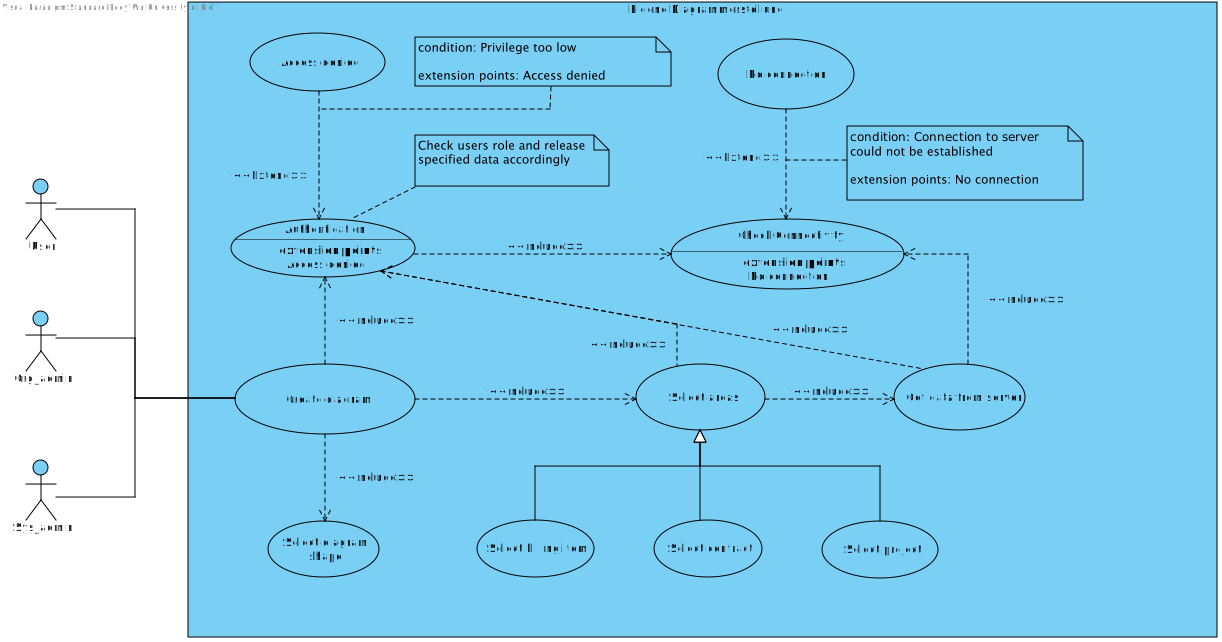
\includegraphics[width=\linewidth]{img/diagrams/Create_Custom_Diagram.pdf.svg}
	\caption{Anwendungsfalldiagramm - Diagrammerstellung}
	\label{fig:anwendungsfalldiagramm-dia-erstellung}
\end{figure}

\newpage

\begin{figure}[h]
	\centering
	\begin{tabularx}{\textwidth}{ X | X }
		\textbf{Anwendungsfall ID} & DIA-2 \\ \hline
		\textbf{Anwendungsfallname} & Diagrammerstellung\\ \hline
		\textbf{Initiierender Akteur} & Mitarbeiter, Org-Admin, Sys-Admin \\ \hline
%		\textbf{Weitere Akteure} & Organisationsadministrator, Mitarbeiter \\ \hline
		\textbf{Kurzbeschreibung} & Nutzer der Weboberfläche können aus den für sie lesbaren Daten auf dem Server, aus den Bereichen Leistungsposition, Vertrag und Projekt, Diagramme in unterschiedlichen Darstellungen erstellen.  \\ \hline
		\textbf{Vorbedingungen} & Der Nutzer hat Zugriffsrechte auf die zu visualisierenden Daten.  \\ \hline
		\textbf{Nachbedingungen} &  Dem Nutzer wird das angefragte Diagramm angezeigt.  \\ \hline
		\textbf{Ablauf} &
		\begin{enumerate}
			\item Der Benutzer loggt sich in der Weboberfläche mit den Benutzerdaten, bestehend aus Benutzername und Passwort, ein.
			\item Der Benutzer wählt eine Diagramm-Darstellung .
			\item Der Benutzer wählt aus einer Liste Leistungspositionen, Verträge und Projekte aus auf die er Zugriff hat und die er im Diagramm visualisieren möchte.
			\item Es wird eine Anfrage an den Server bezüglich der Übermittlung der Daten geschickt.
			\item Das Diagramm wird dem Benutzer angezeigt.
		\end{enumerate} \\ \hline

		\textbf{Alternative} & - \\ \hline
	\end{tabularx}
	\caption{Anwendungsfall DIA-2}
	\label{fig:anwendungsfall-DIA-2}
	
	
\end{figure}


\newpage

\begin{figure}[h]
	\centering
	\begin{tabularx}{\textwidth}{ X | X }
		\multirow{2}{*}{\textbf{Ausnahmen}} &
		\begin{enumerate} % Nutzer wählt Daten aus ohne Zugriffsrecht / während der Bereich-auswahl
			\item Der Benutzer loggt sich in der Weboberfläche mit den Benutzerdaten, bestehend aus Benutzername und Passwort, ein.
			\item Der Benutzer wählt eine Diagramm-Darstellung .
			\item Der Benutzer wählt aus einer Liste Leistungspositionen, Verträge und Projekte aus auf die er Zugriff hat und die er im Diagramm visualisieren möchte.
			\item Es wird eine Anfrage an den Server bezüglich der Übermittlung der Daten geschickt.
			\item Der Server verweigert den Zugriff auf die Daten durch fehlende Zugriffsrechte.
		\end{enumerate} \\\cline{2-2} &
		\begin{enumerate} % Verbindungsfehler
			\item Der Benutzer loggt sich in der Weboberfläche mit den Benutzerdaten, bestehend aus Benutzername und Passwort, ein.
			\item Der Benutzer wählt eine Diagramm-Darstellung .
			\item Der Benutzer wählt aus einer Liste Leistungspositionen, Verträge und Projekte aus auf die er Zugriff hat und die er im Diagramm visualisieren möchte.
			\item Es wird eine Anfrage an den Server bezüglich der Übermittlung der Daten geschickt.
			\item Verbindungsfehler
		\end{enumerate}  \\ \hline
		\textbf{Benutzte Anwendungsfälle} & Benutzerverwaltung (ACC-1), Diagrammverwaltung (DIA-1)\\ \hline
		\textbf{Spezielle Anforderungen} & - \\ \hline
		\textbf{Annahmen} & -
	\end{tabularx}
	\caption{Anwendungsfall DIA-2}
	\label{fig:anwendungsfall-DIA-2}
\end{figure}

	\chapter{Testfälle}\label{chp:testfaelle}
	\centering
\begin{longtable}[c]{|p{1cm}|p{3cm}|p{4cm}|p{6cm}|}
    \caption{Beschreibung der Testfälle}
    \label{fig:testfälle}
    \endlastfoot
    \hline \multicolumn{4}{|r|}{{Weitergeführt auf der folgenden Seite}}                                                                                                                                                                                                                                                                        \\ \hline
    \endfoot
    \hline
    \textbf{Nr.} & \textbf{Anwendungsfall ID} & \textbf{Szenario}                                                                                                  & \textbf{Erwartetes Verhalten}                                                                                                                                              \\ \hline
    \endhead
    \hline
    01           & APP-1                      & Der User loggt sich in die Applikation mit seinen Daten ein.                                                       & Der AppUser erhält eine Übersicht über seine Projekte.   \\ \hline                                                                                                                                                                                                                                                                                                               \\ \hline
    %%---- APP-1: Ablauf ----%%
    02           & APP-1                      & Der User weist einer Leistungsposition einen neuen Status zu.                                                     & Der neue Status wird dem Server mitgeteilt und ist für befugte User sichtbar. Falls keine Verbindung zum Server besteht, wird der neue Status lokal zwischengespeichert. \\ \hline
    %%---- APP-1: Alternative 1 ----%%
    03           & APP-1                      & Ein Bild wird einer Leistungsposition vom AppUser zugeordnet.                                                       & Das Bild wird als Review auf den Server geladen und ist für einen Befugten sichtbar. Falls keine Verbindung zum Server besteht, wird das Bild lokal zwischengespeichert.   \\ \hline
    04           & APP-1                      & Der befugte AppUser will den aktuellen Status einer Leistungsposition einsehen.                                     & Es wird der aktuelle Status der gewählten Leistungsposition angezeigt.                                                                                                     \\ \hline
    05           & APP-1                      & Der AppUser trägt seinen Nutzernamen, sein Passwort und die gültige URL des WebServers ein.                        & Eine neue Verbindung zu einem WebServer wird hergestellt.                                                                                                                  \\ \hline
    00           & ACC-1                      & Der WebUser loggt sich in die Applikation mit seinen Daten ein.                                                    & Der SysAdmin erhält eine Übersicht über die Organisationen. Der OrgAdmin und B.m.b.R. erhalten eine Übersicht der Verträge. \\ \hline
    06           & ACC-1                      & Der OrgAdmin erstellt eine neue Rolle mit gewählten Rechten.                                                       & Die neue Rolle ist erstellt und hat die gewählten Rechte für bestimmte Bereiche auf dem WebServer.                                                                         \\ \hline
    07           & ACC-1                      & Der OrgAdmin fügt neue User hinzu oder löscht bestehende.                                                        & Neue User werden dauerhaft Organisationen mit einer Rolle zugewiesen. Zu löschende User werden dauerhaft aus der Organisation gelöscht.                                \\ \hline
    08           & ACC-1                      & Der SysAdmin erstellt eine neue Organisation mit zugehörigen OrgAdmins.                                            & Nach Erstellung der Organisationen können die OrgAdmins beliebig User hinzufügen, bearbeiten oder löschen.                                                               \\ \hline
    %%---- ACC-1: Ablauf ----%%
    09           & ACC-1                      & B.m.b.R. bearbeitet Leistungspositionen.                                                                           & Daten der Leistungsposition können erfolgreich modifiziert und dauerhaft gespeichert werden.                                                                               \\ \hline
    10           & ACC-1                      & B.m.b.R. hat Einsicht in die Vertragsdaten.                                                                        & Aus dieser Übersicht können Diagramme erstellt und Vertragsdaten geändert werden.                                                                                          \\ \hline
    %%---- DIA-1: Ablauf ----%%
    11           & DIA-1                      & B.m.b.R. wählt ein alle Leistungspositionen umfassendes Diagramm eines oder mehrerer Verträge zur Darstellung.     & Das passende Diagramm wird angezeigt.                                                                                                                                      \\ \hline
    12           & DIA-1                      & B.m.b.R. lädt die Vertragsdaten mit den Diagrammen oder die Leistungspositionen.                                   & Es werden automatisch passende Diagramme erzeugt.                                                                                                                          \\ \hline
    %%---- DIA-1: Alternative 1 ----%%
    13           & DIA-1                      & B.m.b.R. nutzt die Filterfunktion bei den Vertragsdaten, Projekten und Leistungspositionen.                        & Die Ergebnisse werden nach dem entsprechenden Kriterium gefiltert angezeigt.                                                                                               \\ \hline
    %%---- DIA-1: Alternative 2 ----%%
    14           & DIA-1                      & B.m.b.R. wählt ein Diagramm zum Baufortschritt eines bestimmten Projektes.                                         & Das gewählte Diagramm wird angezeigt.                                                                                                                                      \\ \hline
    %%---- DIA-2: Ablauf ----%%
    15           & DIA-2                      & B.m.b.R. wählt aus einer Liste Leistungspositionen, Verträge und Projekte aus, um ein Diagramm erstellen zu lassen. & Es wird ein zur Auswahl passendes Diagramm erstellt.                                                                                                                      \\ \hline
\end{longtable}
	
	\chapter{Produktdaten}\label{chp:produktdaten}
	\section{Webserver}

Referenzielle Daten werden nicht explizit gelistet, wenn sie ohnehin schon in der Applikation an anderer Stelle gespeicher, bwz. genutzt werden.
Ein Beispiel hierfür sind Projekte und dazugehörige Leistungspositionen. Für die Projektdaten werden hier also keine IDs von zugehörigen Leistungspositionen
als Produkdaten aufgeführt, das diese IDs nur als Referenz genutzt werden und bereits in den Leistungspositionsdaten aufgeführt werden.

\subsection{Übersicht Benutzerrollen}

\begin{figure}[h]
	\centering
	\begin{tabularx}{\textwidth}{| X | X |}
        \hline
		\textbf{Benutzerrolle} & \textbf{ID} \\ \hline \hline
		\textbf{Systemadministrator} & SysAdmin \\ \hline
		\textbf{Organisationsadministrator} & OrgAdmin \\ \hline
        \textbf{Allgemeiner Nutzer der Webapplikation} & User \\ \hline
		\textbf{Andere Nutzerrolle innerhalb einer Organisation} & OrgUser \\ \hline
	\end{tabularx}
	\caption{Benutzerrollen}
	\label{fig:Benutzerrollen}
\end{figure}

\begin{flushleft}
Es werden nur allgemeine Rollen beschrieben. Organisationsadministratoren können eigene Rollen beschreiben und zuweisen. Diese verhalten sich allgemein wie die Rolle \textbf{OrgUser}.
Ein \textbf{OrgUser} kann z.Bsp. nur Daten einer Leistungsposition einsehen, sofern seine Rolle innerhalb seiner Organisation dies zulässt. Ebenso können \textbf{OrgAdmin} beispielsweise nur Verträge und
Positionen ihrer jeweiligen Organisation einsehen.
\end{flushleft}

\subsection{Benutzerdaten}

Die Benutzerdaten umfassen alle Informationen zu einem registrierten Benutzer der Webanwendung. Diese Daten sind nur f\"ur den Benutzer selbst und f\"ur Systemadministratoren einsehbar.

\begin{figure}[h]
	\centering
	\begin{tabularx}{\textwidth}{| X || X | X |}
        \hline
		\textbf{Art der Daten} & \textbf{Beschreibung der Daten} & \textbf{Zugriffsberechtigung} \\ \hline \hline
		\textbf{Benutzerkennung} & Eindeutiger Benutzername und ein Passwort(Hash) & SysAdmin, zugehöriger User (nur Benutzername) \\ \hline
		\textbf{Persönliche Daten} & Name, Nachname und Organisation & SysAdmin, zugehöriger OrgAdmin, zugehöriger User \\ \hline
		\textbf{Benutzerrolle} & Rolle des Benutzers & SysAdmin, zugehöriger OrgAdmin, zugehöriger User \\ \hline
	\end{tabularx}
	\caption{Benutzerdaten}
	\label{fig:Benutzerdaten}
\end{figure}

\newpage

\subsection{Projektdaten}

Die Projektdaten setzen sich aus den Daten der zur Verf\"ugung gestellten REST-API zusammen.

\begin{figure}[h]
	\centering
	\begin{tabularx}{\textwidth}{| X || X | X |}
        \hline
		\textbf{Art der Daten} & \textbf{Beschreibung der Daten} & \textbf{Zugriffsberechtigung} \\ \hline \hline
        \textbf{ID} & ID des Projekts & SysAdmin \\ \hline
		\textbf{Projektname} & Name des Projekts & SysAdmin, zugehöriger OrgAdmin, zugehöriger OrgUser \\ \hline
		\textbf{Projektbeschreibung} & Projektbeschreibungg & SysAdmin, zugehöriger OrgAdmin, zugehöriger OrgUser \\ \hline
		\textbf{Fertigstellungsdatum} & Datum der geplanten Fertigstellung & SysAdmin, zugehöriger OrgAdmin, zugehöriger OrgUser \\ \hline
        \textbf{Adresse} & Adresse/Ort des Projekts & SysAdmin, zugehöriger OrgAdmin, zugehöriger OrgUser \\ \hline
	\end{tabularx}
	\caption{Projektdaten}
	\label{fig:Projektdaten}
\end{figure}

\subsection{Vertragsdaten}

Die Vertragsdaten setzen sich aus den Daten der zur Verf\"ugung gestellten REST-API zusammen. Vertragsdaten werden pro Vertrag gespeichert.

\begin{figure}[h]
	\centering
	\begin{tabularx}{\textwidth}{| X || X | X |}
        \hline
		\textbf{Art der Daten} & \textbf{Beschreibung der Daten} & \textbf{Zugriffsberechtigung} \\ \hline \hline
		\textbf{VertragsID} & ID des Vertrages & SysAdmin \\ \hline
		\textbf{Vertragsname} & Name des Vertrages & SysAdmin, zugehöriger OrgAdmin \\ \hline
	\end{tabularx}
	\caption{Vertragsdaten}
	\label{fig:Vertragsdaten}
\end{figure}

\newpage

\subsection{Leistungspositionsdaten}

Die Leistungspositionsdaten setzen sich aus den Daten der zur Verf\"ugung gestellten REST-API zusammen und aus dem Status einer jeweiligen Position, welcher über die mobile Applikation geändert werden kann.
Sie werden pro Leistungsposition gespeichert.

\begin{figure}[h]
	\centering
	\begin{tabularx}{\textwidth}{| X || X | X |}
        \hline
		\textbf{Art der Daten} & \textbf{Beschreibung der Daten} & \textbf{Zugriffsberechtigung} \\ \hline \hline
		\textbf{PositionsID} & ID des Vertrages & SysAdmin \\ \hline
		\textbf{Status} & Name des Vertrages & SysAdmin, zugehöriger OrgAdmin, zugehöriger OrgUser \\ \hline
		\textbf{Qualitätsicherungsdaten} & Fotos und dazugehörige Kommentare & SysAdmin, zugehöriger OrgAdmin, zugehöriger OrgUser \\ \hline
	\end{tabularx}
	\caption{Leistungspositionsdaten}
	\label{fig:Leistungspositionsdaten}
\end{figure}
	
	\chapter{Benutzeroberfläche}\label{chp:benutzeroberflaeche}
	
\begin{figure}[h]
\centering
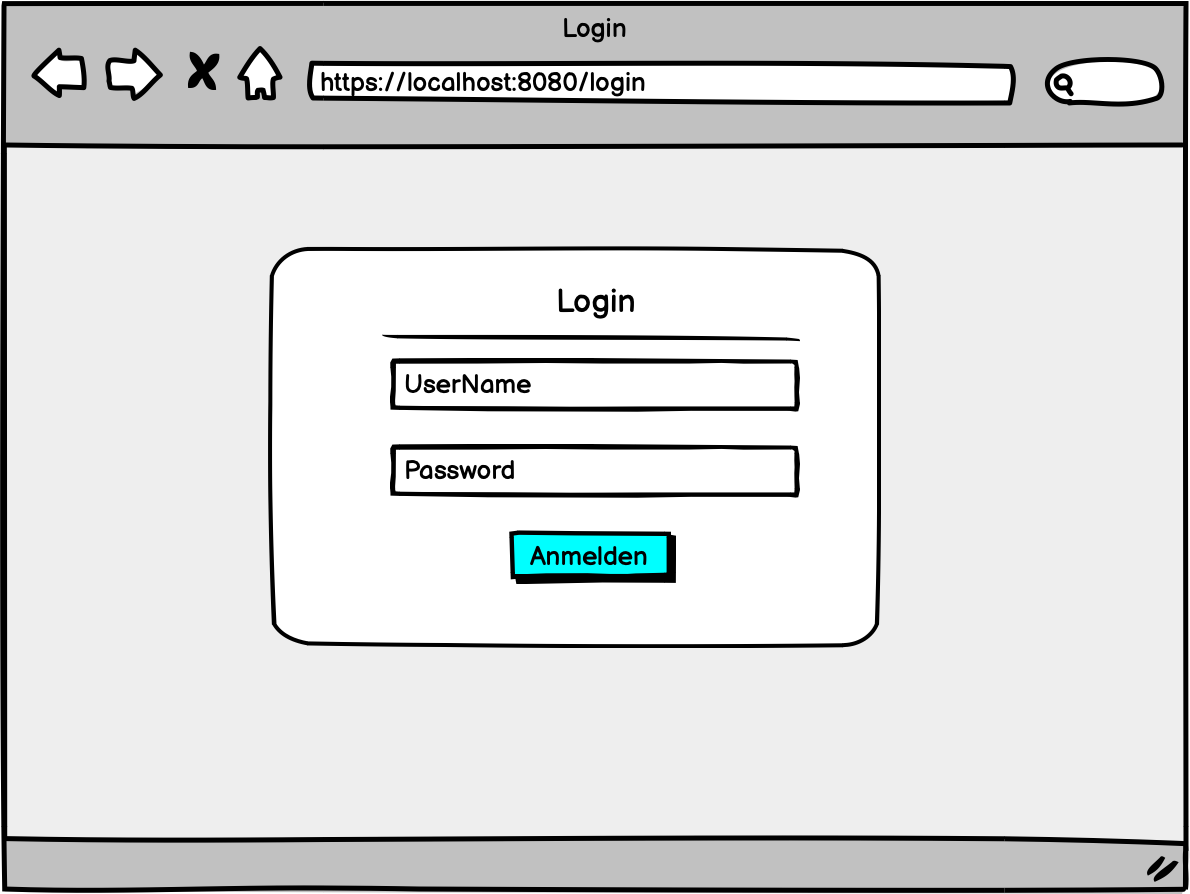
\includegraphics[width=10cm]{img/mockup_web/login.png}
\caption{Login-Seite - Sie ist für alle Benutzer sichtbar.}
\end{figure}

\begin{figure}[h]
\centering
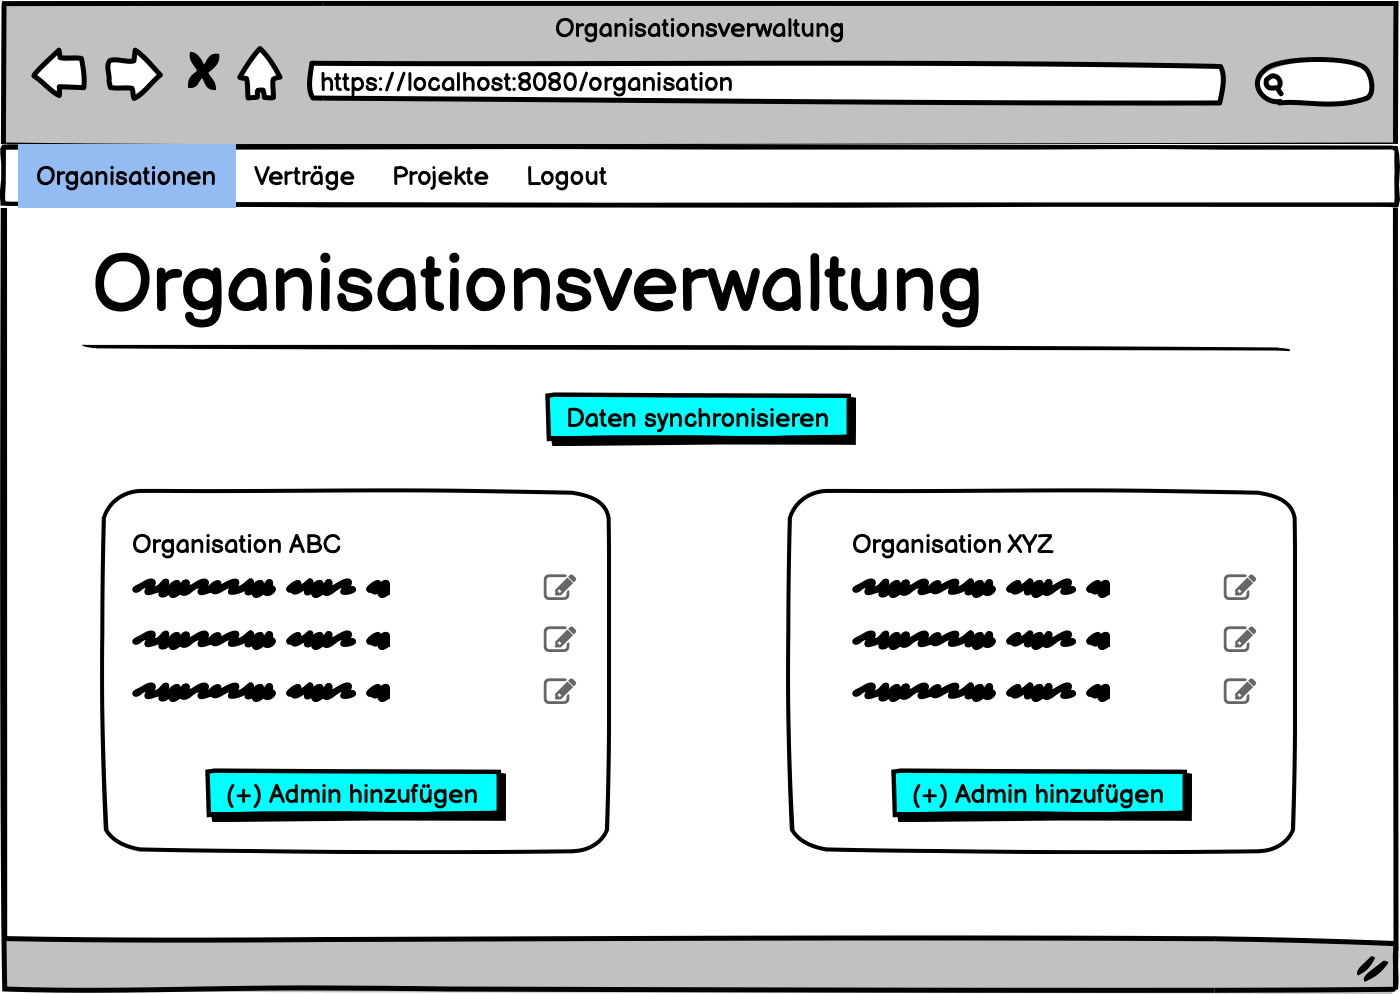
\includegraphics[width=10cm]{img/mockup_web/system-admin-orgs.png}
\caption{Verwaltung der Organisationen und deren Admins - Sichtbar nur für die Systemadmins.}
\end{figure}

\begin{figure}[h]
\centering
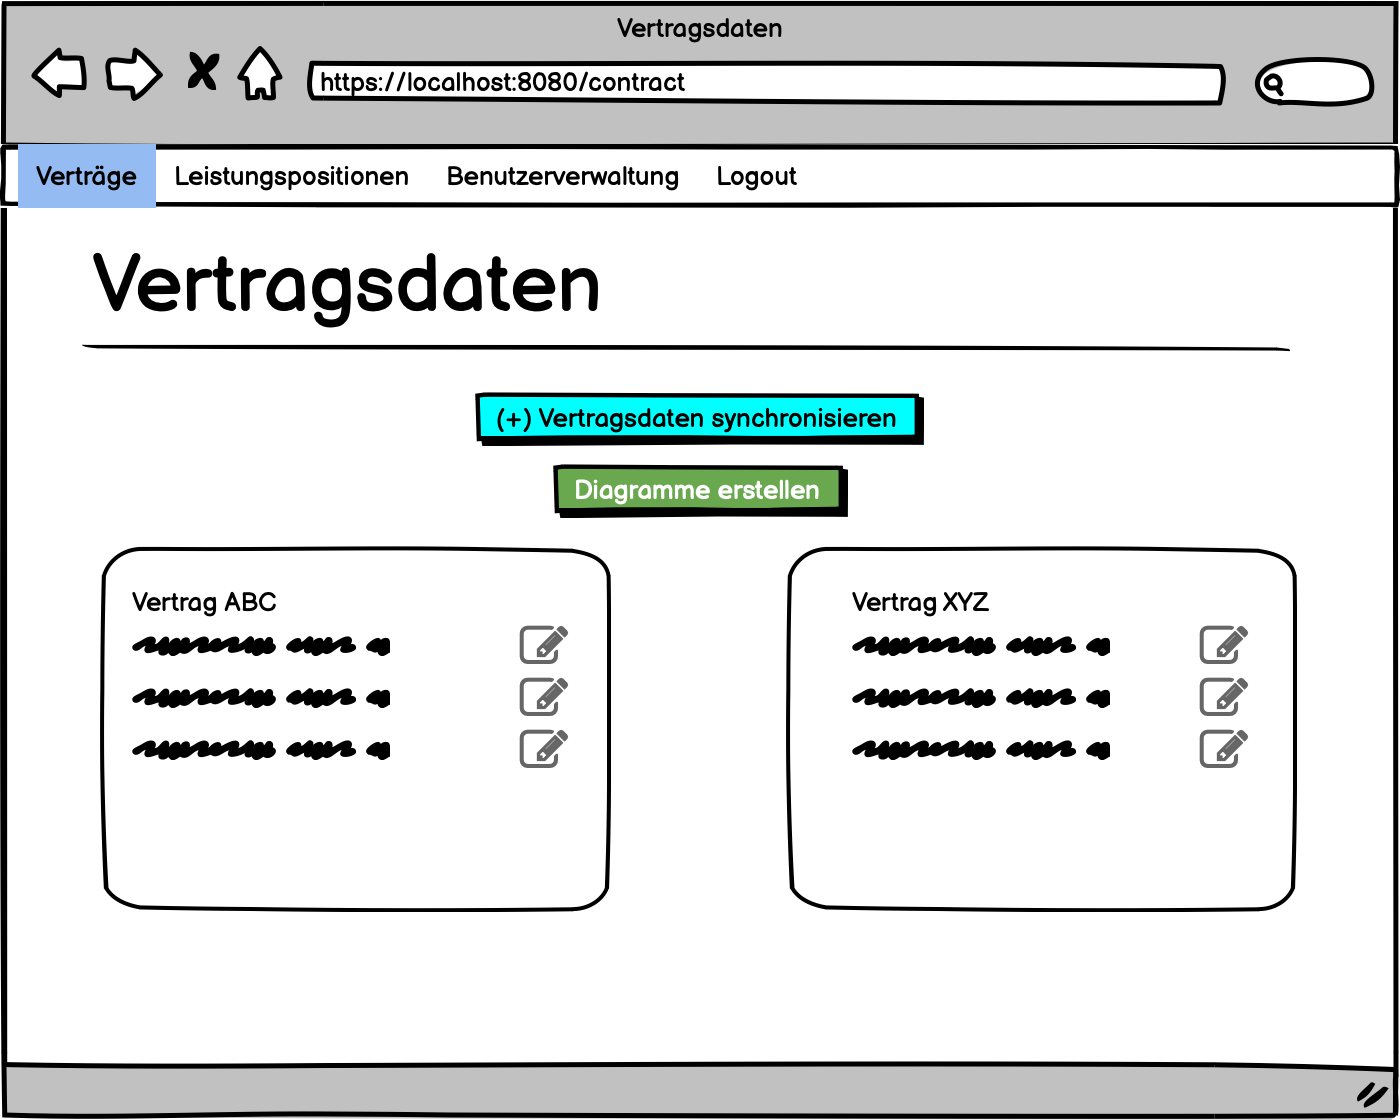
\includegraphics[width=10cm]{img/mockup_web/admin-vertraege.png}
\caption{Übersicht über die Verträge - Nur die (System-)Admins können diese einsehen.}
\end{figure}

\begin{figure}[h]
\centering
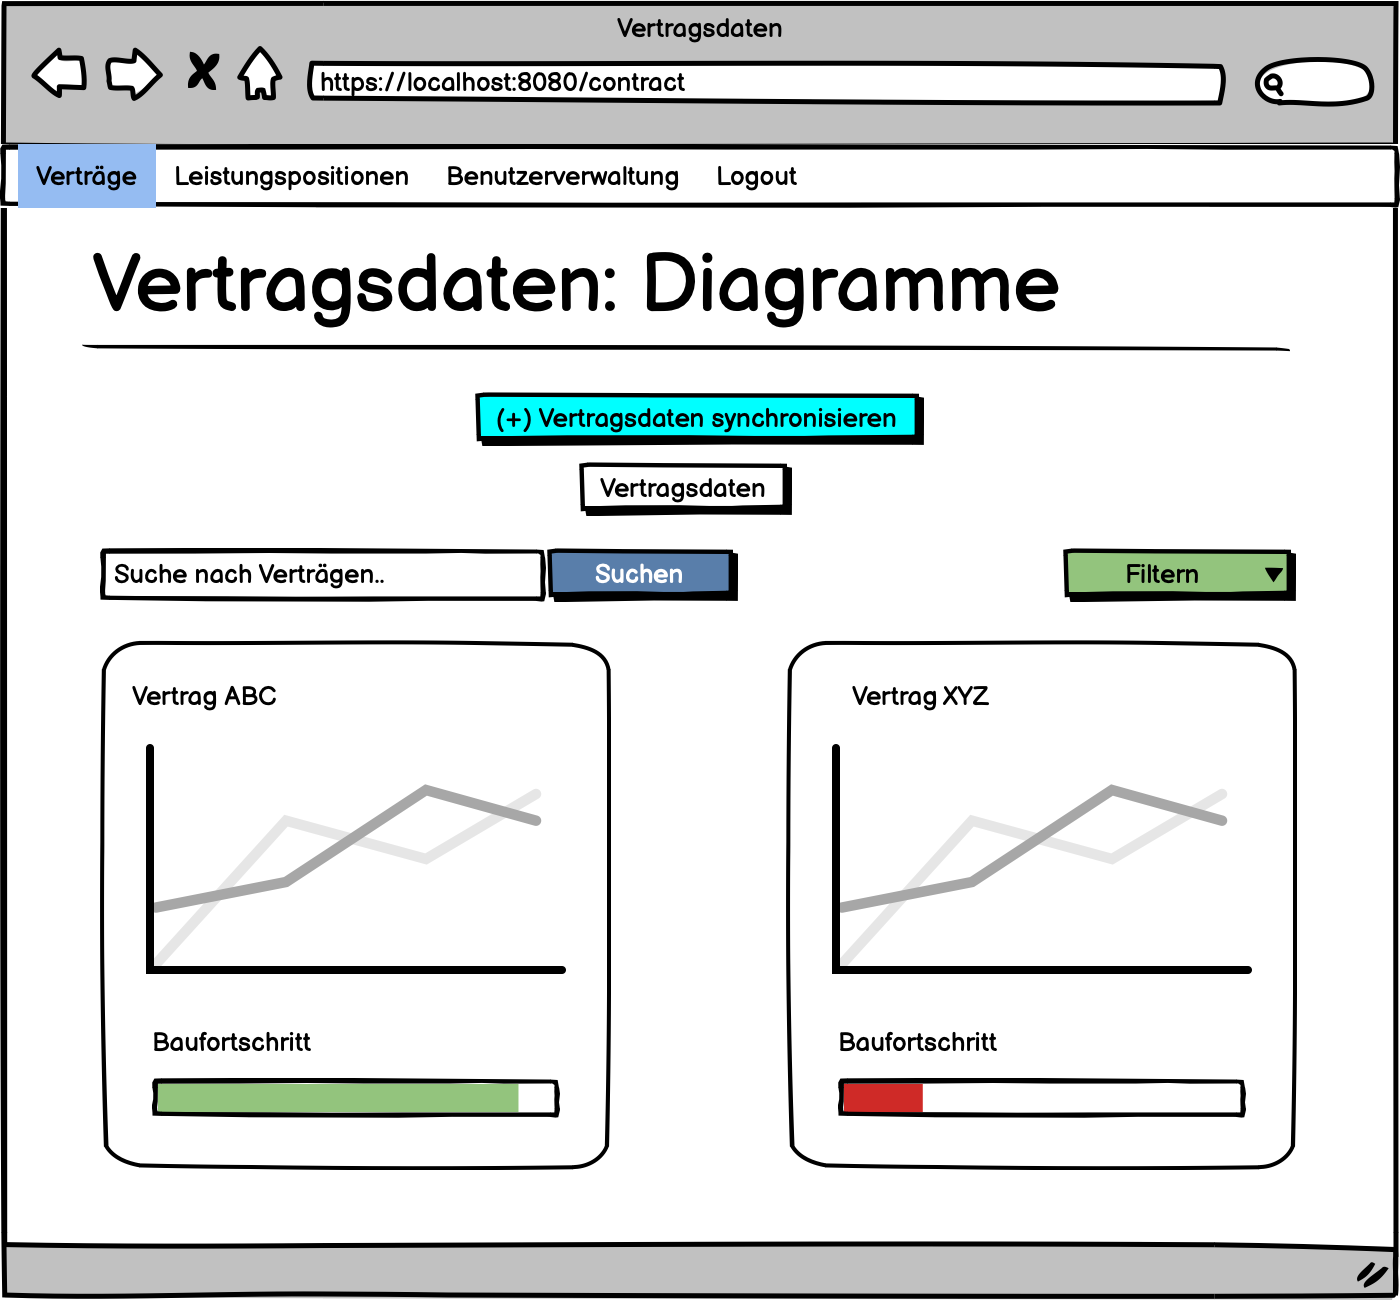
\includegraphics[width=10cm]{img/mockup_web/admin-vertraege-diagramme.png}
\caption{Übersicht über die Verträge mit Diagrammen - Nur die (System-)Admins können diese einsehen.}
\end{figure}

\begin{figure}[h]
\centering
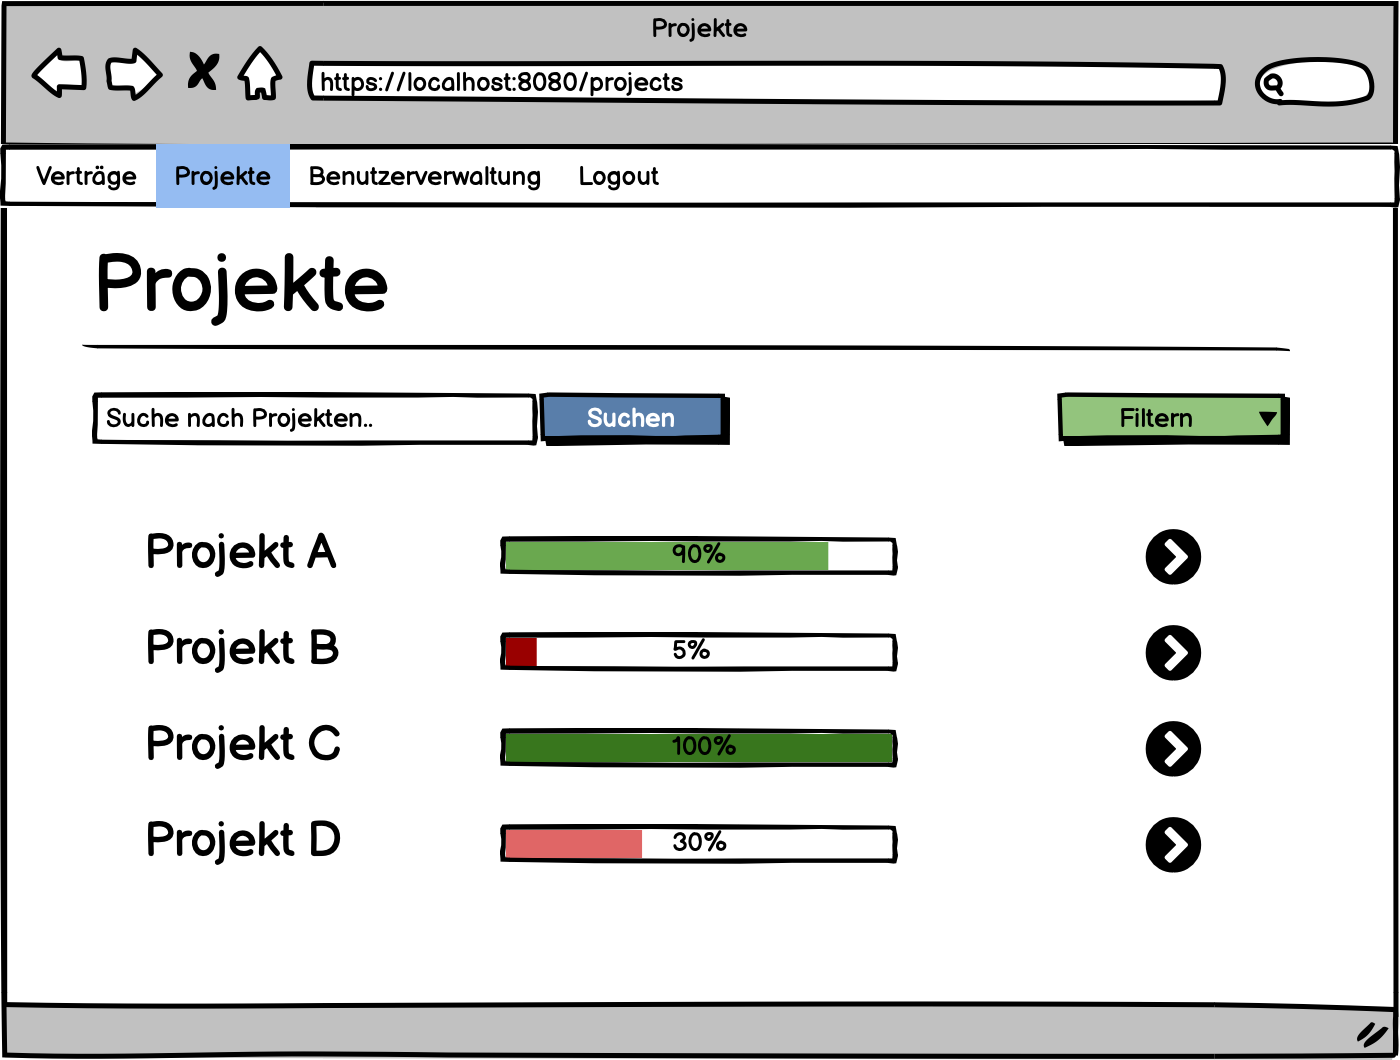
\includegraphics[width=10cm]{img/mockup_web/admin-und-benutzer-projekte.png}
\caption{Übersicht der Projekte - Sichtbar für Benutzer und (System-)Admins}
\end{figure}

\begin{figure}[h]
\centering
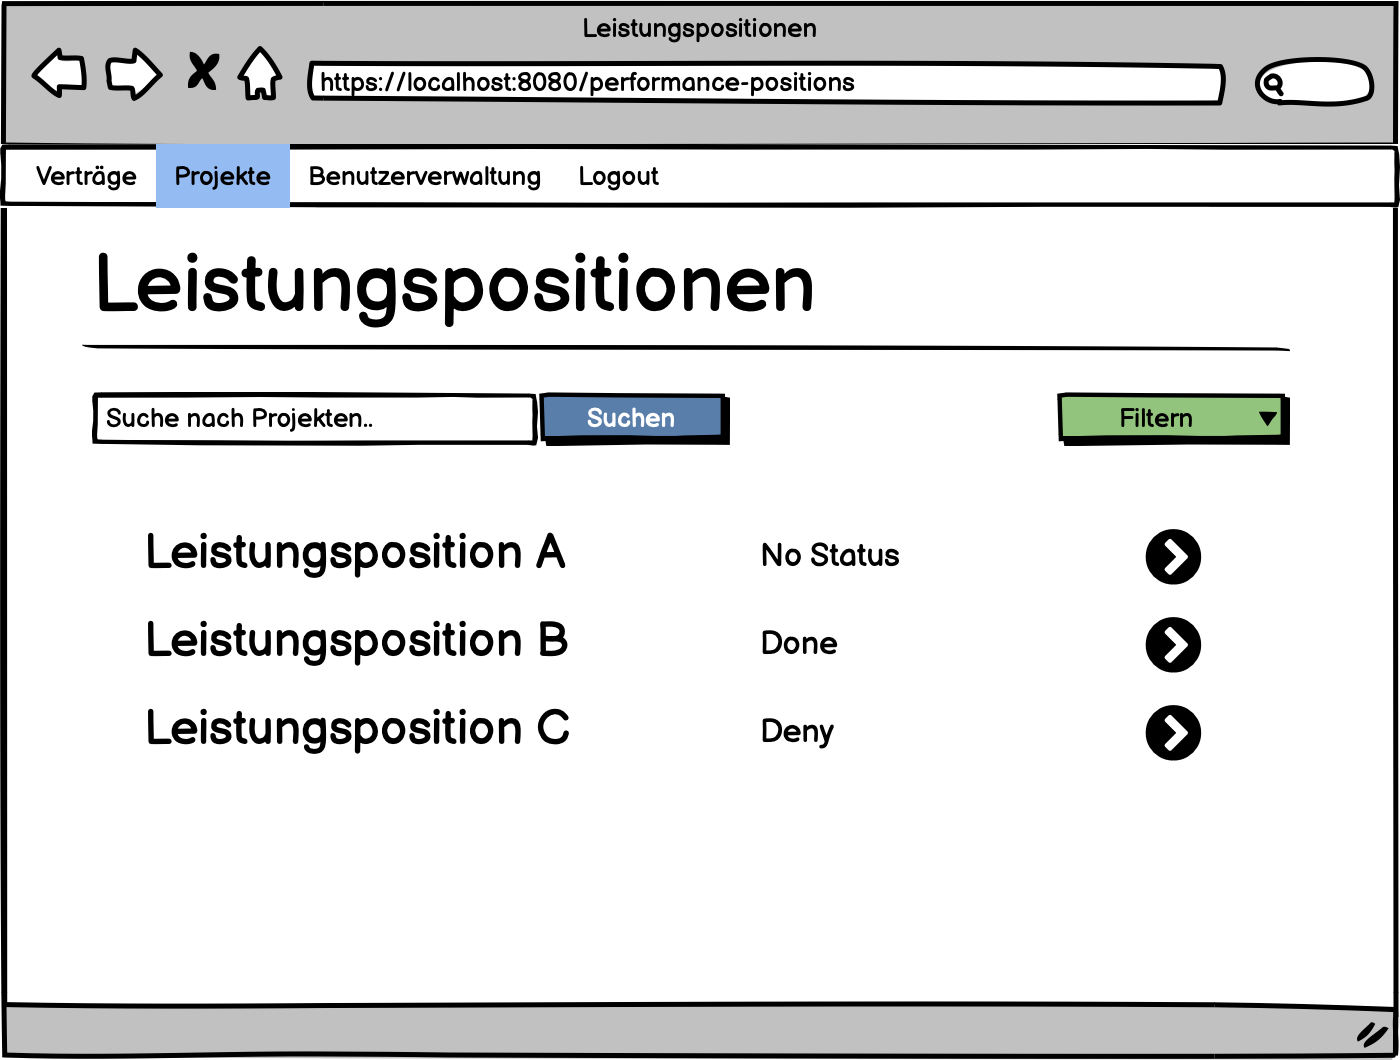
\includegraphics[width=10cm]{img/mockup_web/admin-und-benutzer-leistungspositionen.png}
\caption{Übersicht der Leistungspositionen - Sichtbar für Benutzer und (System-)Admins}
\end{figure}

\begin{figure}[h]
\centering
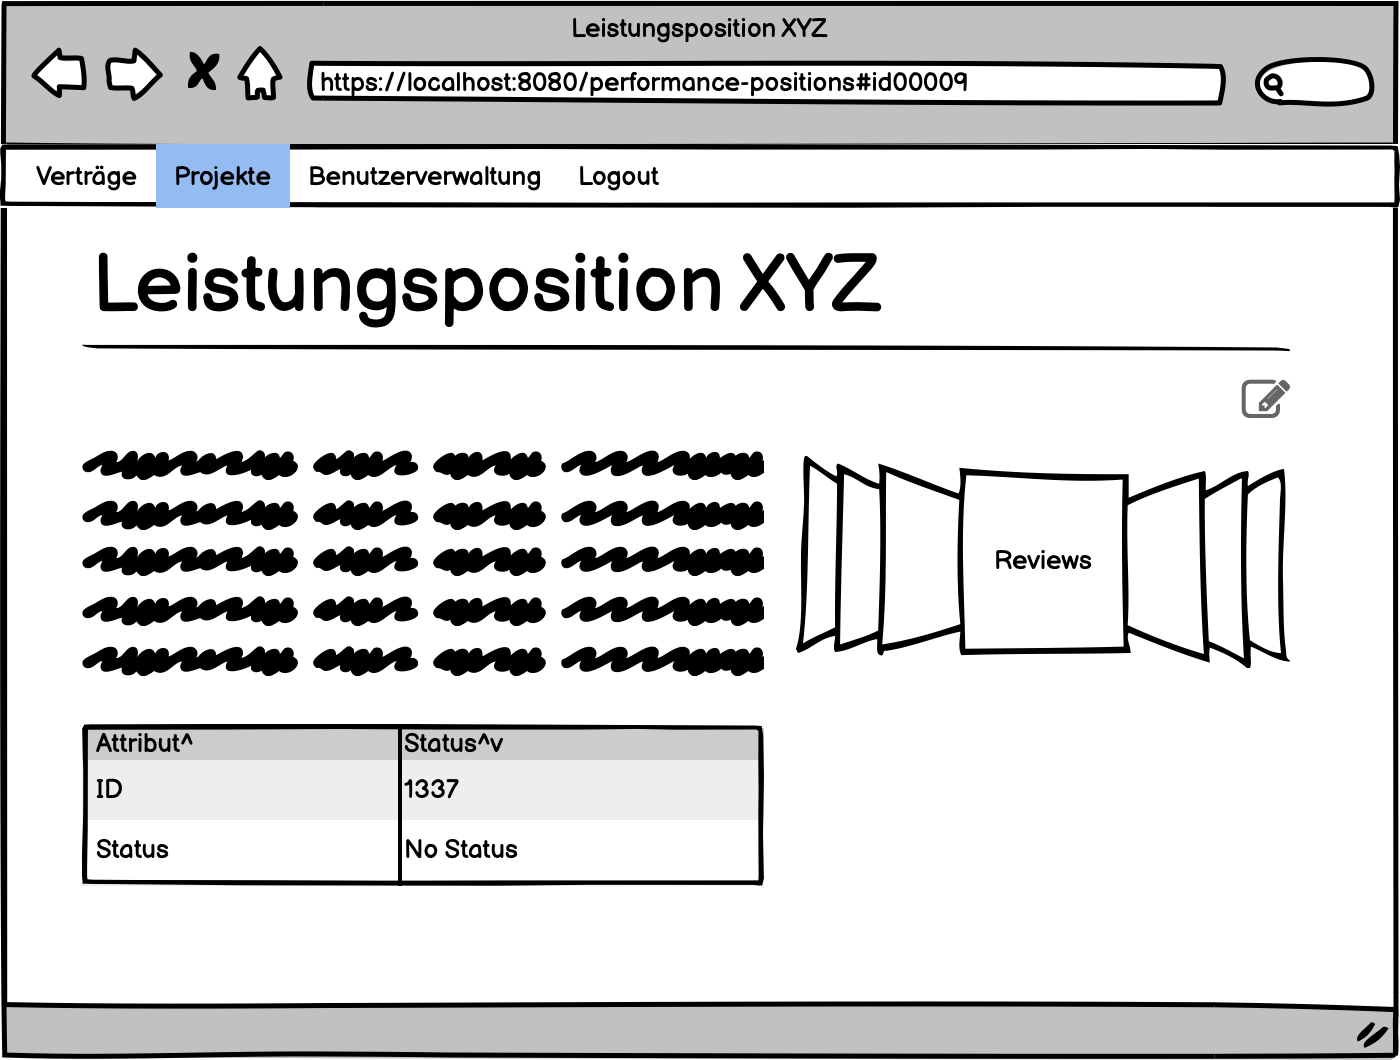
\includegraphics[width=10cm]{img/mockup_web/admin-und-benutzer-leistungsposition-exmpl.png}
\caption{Übersicht eienr bestimmten Leistungsposition - Sichtbar für Benutzer und (System-)Admins}
\end{figure}

\begin{figure}[h]
\centering
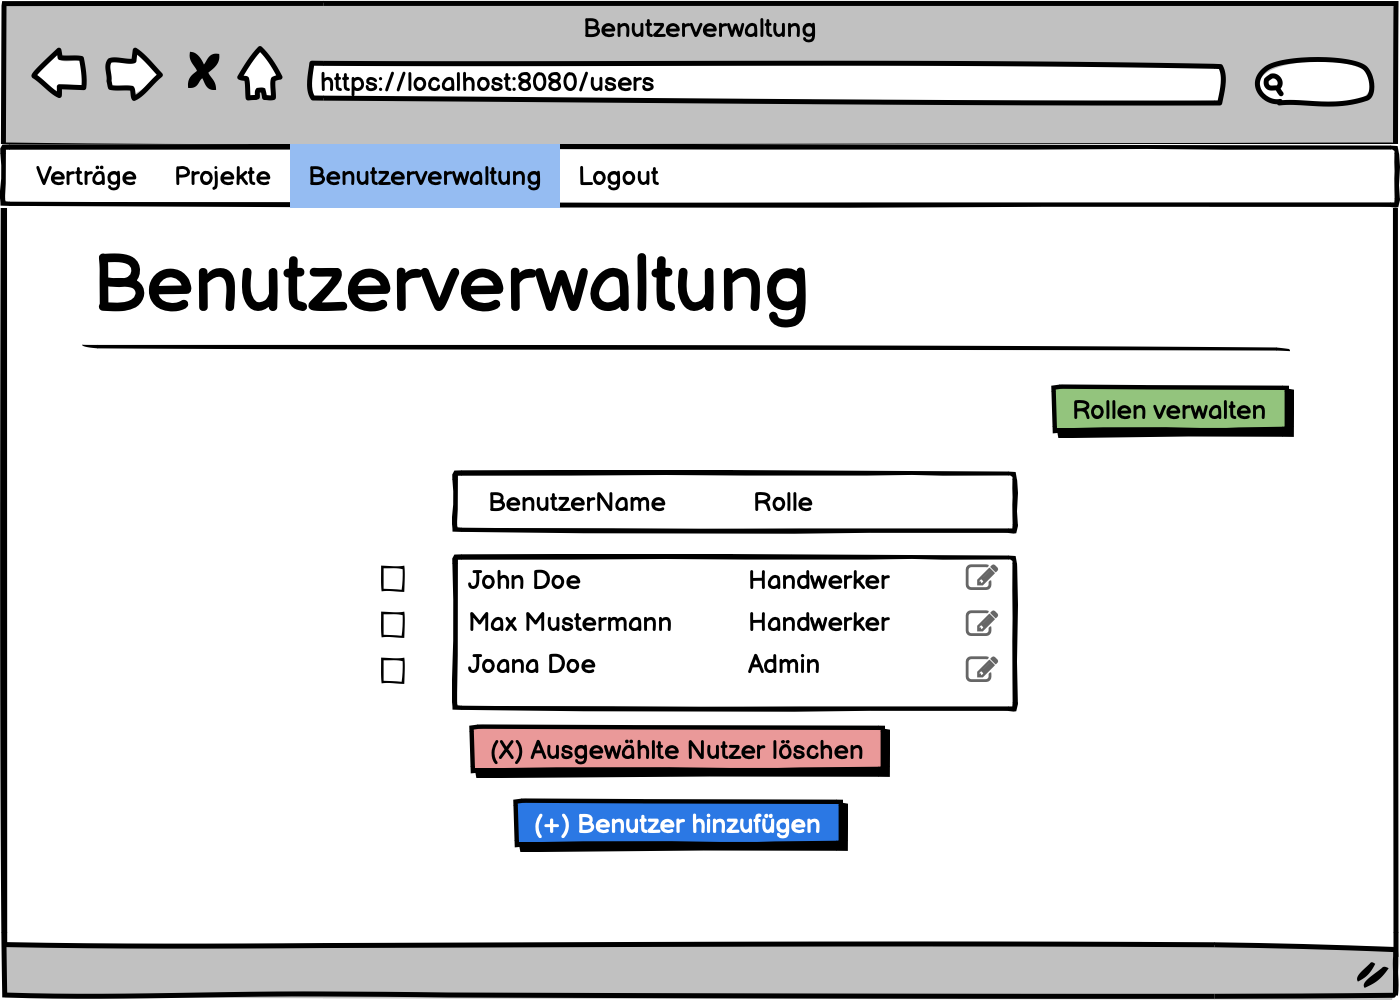
\includegraphics[width=10cm]{img/mockup_web/admin-und-benutzer-benutzerverwaltung.png}
\caption{Benutzerverwaltung - Sichtbar nur für (System-)Admins}
\end{figure}

\begin{figure}[h]
\centering
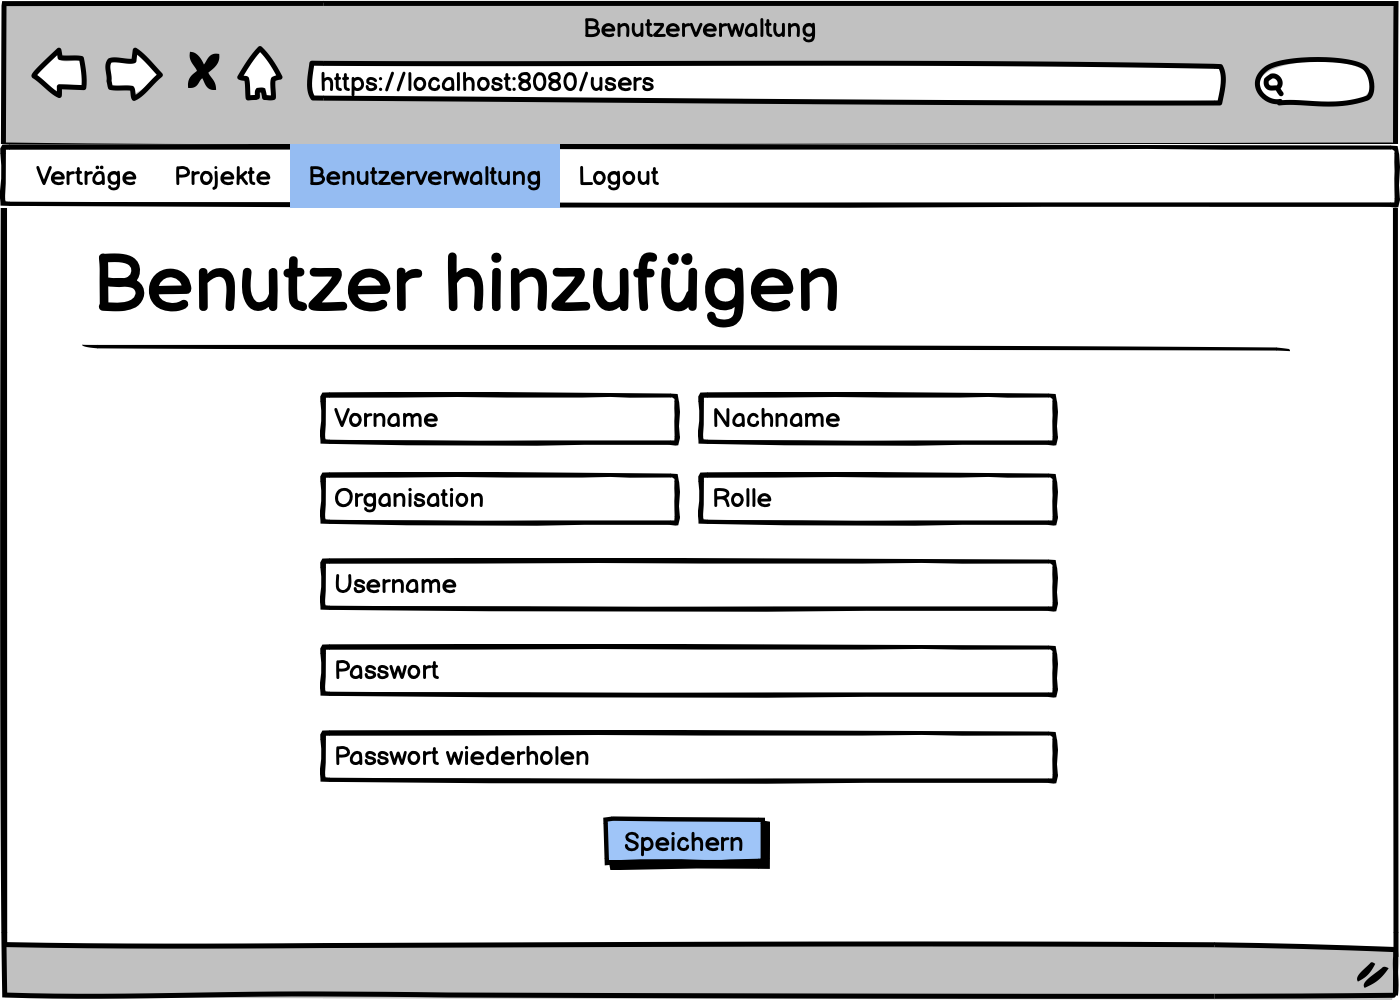
\includegraphics[width=10cm]{img/mockup_web/admin-und-benutzer-erstellen.png}
\caption{Benutzer erstellen - Nur sichtbar für (System-)Admins.}
\end{figure}
	
	\chapter{Glossar}\label{chp:glossar}
	\begin{tcolorbox}
	In diesem Glossar können Akronyme und abkürzende Schreibweisen aufgelistet werden. 
	Alle verwendeten Abkürzungen innerhalb des Projekts müssen hier erläutert werden.
\end{tcolorbox}

\begin{table}[h]
	\centering
	\begin{tabularx}{\textwidth}{X X}
		\rowcolor[HTML]{C0C0C0} 
		\textbf{Abkürzung} & \textbf{Beschreibung} \\
		Anwendungsadministrator, sysadmin & Systemadministrator \\

		\rowcolor[HTML]{E7E7E7} 
		API & Application Programming Interface
		Applikation & App \\

		\rowcolor[HTML]{E7E7E7} 
		Appuser & Benutzer der Android App \\
		
		Authentifizierung & Verifizierung der Identität auf dem server \\
		
		\rowcolor[HTML]{E7E7E7} 
		Berechtigung & Zugriffsrechte wie z.B. lesen und Schreiben von Daten \\
		BillingItem & Leistungsposition \\
		GUI & Graphical User Interface \\

		\rowcolor[HTML]{E7E7E7} 
		orgadmin & Organisationsadministrator \\
		Organisationsadministrator & Hat Zugriff auf alle Daten und Mitarbeiter in einer Organisation \\
		\rowcolor[HTML]{E7E7E7} 
		OrgUser & Nutzer der einer Organisation zugeordnet ist \\
		
		REST-API & Eine Programmierschnittstelle (API) die HTTP-Anfragen verwendet um per GET, PUT, POST, und DELETE auf Daten zuzugreifen.\\
		\rowcolor[HTML]{E7E7E7} 
		user & Benutzer \\
	\end{tabularx}
	\caption{Glossar}
	\label{table:glossar}
\end{table}
	
	\bibliography{references}
	\pagenumbering{gobble} % Nummerierung deaktivieren
	
\end{document}
